% This must be in the first 5 lines to tell arXiv to use pdfLaTeX, which is strongly recommended.
\pdfoutput=1
% In particular, the hyperref package requires pdfLaTeX in order to break URLs across lines.

\documentclass[11pt]{article}

% Change "review" to "final" to generate the final (sometimes called camera-ready) version.
% Change to "preprint" to generate a non-anonymous version with page numbers.
% \usepackage[review]{acl}
% fixed for camera-ready
\usepackage[final]{acl}

% Standard package includes
\usepackage{times}
\usepackage{latexsym}

% For proper rendering and hyphenation of words containing Latin characters (including in bib files)
\usepackage[T1]{fontenc}
% For Vietnamese characters
% \usepackage[T5]{fontenc}
% See https://www.latex-project.org/help/documentation/encguide.pdf for other character sets

% This assumes your files are encoded as UTF8
\usepackage[utf8]{inputenc}

% This is not strictly necessary, and may be commented out,
% but it will improve the layout of the manuscript,
% and will typically save some space.
\usepackage{microtype}

% This is also not strictly necessary, and may be commented out.
% However, it will improve the aesthetics of text in
% the typewriter font.
\usepackage{inconsolata}

%Including images in your LaTeX document requires adding
%additional package(s)
\usepackage{graphicx}
\usepackage{subcaption}

% % by Sumin
% \usepackage{pifont}
% \usepackage{multirow}
\usepackage{booktabs}
\usepackage{amssymb,amsmath,amsthm}
\usepackage{bm}
\usepackage{pifont}
\usepackage{multirow}
% \usepackage{subfigure}
\setlength{\abovedisplayskip}{10pt} % Space above equations
\setlength{\belowdisplayskip}{10pt} % Space below equations



\newcommand{\etal}{\textit{et al}. }
\newcommand{\ie}{\textit{i}.\textit{e}., }
\newcommand{\eg}{\textit{e}.\textit{g}., }

\newcommand{\phseo}[1]{\textcolor{blue}{[Paul: #1]}}
\newcommand{\sumin}[1]{\textcolor{orange!85!black}{[Sumin: #1]}}
\newcommand{\junyoung}[1]{\textcolor{purple}{[Junyoung: #1]}}
\newcommand{\chanjun}[1]{\textcolor{red}{[Chanjun: #1]}}
\newcommand{\model}{LCIRC}

% If the title and author information does not fit in the area allocated, uncomment the following
%
%\setlength\titlebox{<dim>}
%
% and set <dim> to something 5cm or larger.

\title{LCIRC: A Recurrent Compression Approach for Efficient Long-form Context and Query Dependent Modeling in LLMs}

% fixed for camera-ready
\author{
Sumin An\textsuperscript{1} \qquad
Junyoung Sung\textsuperscript{1} \qquad
Wonpyo Park\textsuperscript{2}
\\
\textbf{Chanjun Park\textsuperscript{1,\(\dagger\)}} \qquad
\textbf{Paul Hongsuck Seo\textsuperscript{1,\(\dagger\)}}
\\
\textsuperscript{1}Dept. of CSE, Korea University
\qquad
\textsuperscript{2}Google
\\
\texttt{\{suminan, jys7451, bcj1210, phseo\}@korea.ac.kr}
\\
\texttt{wppark@google.com}
}


\begin{document}
\maketitle
\begin{abstract}
While large language models (LLMs) excel in generating coherent and contextually rich outputs, their capacity to efficiently handle long-form contexts is limited by fixed-length position embeddings. Additionally, the computational cost of processing long sequences increases quadratically, making it challenging to extend context length. 
To address these challenges, we propose Long-form Context Injection with Recurrent Compression (LCIRC), a method that enables the efficient processing long-form sequences beyond the model's length limit through recurrent compression without retraining the entire model.
We further introduce query dependent context modeling, which selectively compresses query-relevant information, ensuring that the model retains the most pertinent content. Our empirical results demonstrate that Query Dependent LCIRC (QD-LCIRC) significantly improves LLM's ability to manage extended contexts, making it well-suited for tasks that require both comprehensive context understanding and query relevance.

\end{abstract}
% fixed for camera-ready
\let\thefootnote\relax\footnotetext{$^\dagger$Co-corresponding authors.}

\section{Introduction}
\label{sec:introduction}
The business processes of organizations are experiencing ever-increasing complexity due to the large amount of data, high number of users, and high-tech devices involved \cite{martin2021pmopportunitieschallenges, beerepoot2023biggestbpmproblems}. This complexity may cause business processes to deviate from normal control flow due to unforeseen and disruptive anomalies \cite{adams2023proceddsriftdetection}. These control-flow anomalies manifest as unknown, skipped, and wrongly-ordered activities in the traces of event logs monitored from the execution of business processes \cite{ko2023adsystematicreview}. For the sake of clarity, let us consider an illustrative example of such anomalies. Figure \ref{FP_ANOMALIES} shows a so-called event log footprint, which captures the control flow relations of four activities of a hypothetical event log. In particular, this footprint captures the control-flow relations between activities \texttt{a}, \texttt{b}, \texttt{c} and \texttt{d}. These are the causal ($\rightarrow$) relation, concurrent ($\parallel$) relation, and other ($\#$) relations such as exclusivity or non-local dependency \cite{aalst2022pmhandbook}. In addition, on the right are six traces, of which five exhibit skipped, wrongly-ordered and unknown control-flow anomalies. For example, $\langle$\texttt{a b d}$\rangle$ has a skipped activity, which is \texttt{c}. Because of this skipped activity, the control-flow relation \texttt{b}$\,\#\,$\texttt{d} is violated, since \texttt{d} directly follows \texttt{b} in the anomalous trace.
\begin{figure}[!t]
\centering
\includegraphics[width=0.9\columnwidth]{images/FP_ANOMALIES.png}
\caption{An example event log footprint with six traces, of which five exhibit control-flow anomalies.}
\label{FP_ANOMALIES}
\end{figure}

\subsection{Control-flow anomaly detection}
Control-flow anomaly detection techniques aim to characterize the normal control flow from event logs and verify whether these deviations occur in new event logs \cite{ko2023adsystematicreview}. To develop control-flow anomaly detection techniques, \revision{process mining} has seen widespread adoption owing to process discovery and \revision{conformance checking}. On the one hand, process discovery is a set of algorithms that encode control-flow relations as a set of model elements and constraints according to a given modeling formalism \cite{aalst2022pmhandbook}; hereafter, we refer to the Petri net, a widespread modeling formalism. On the other hand, \revision{conformance checking} is an explainable set of algorithms that allows linking any deviations with the reference Petri net and providing the fitness measure, namely a measure of how much the Petri net fits the new event log \cite{aalst2022pmhandbook}. Many control-flow anomaly detection techniques based on \revision{conformance checking} (hereafter, \revision{conformance checking}-based techniques) use the fitness measure to determine whether an event log is anomalous \cite{bezerra2009pmad, bezerra2013adlogspais, myers2018icsadpm, pecchia2020applicationfailuresanalysispm}. 

The scientific literature also includes many \revision{conformance checking}-independent techniques for control-flow anomaly detection that combine specific types of trace encodings with machine/deep learning \cite{ko2023adsystematicreview, tavares2023pmtraceencoding}. Whereas these techniques are very effective, their explainability is challenging due to both the type of trace encoding employed and the machine/deep learning model used \cite{rawal2022trustworthyaiadvances,li2023explainablead}. Hence, in the following, we focus on the shortcomings of \revision{conformance checking}-based techniques to investigate whether it is possible to support the development of competitive control-flow anomaly detection techniques while maintaining the explainable nature of \revision{conformance checking}.
\begin{figure}[!t]
\centering
\includegraphics[width=\columnwidth]{images/HIGH_LEVEL_VIEW.png}
\caption{A high-level view of the proposed framework for combining \revision{process mining}-based feature extraction with dimensionality reduction for control-flow anomaly detection.}
\label{HIGH_LEVEL_VIEW}
\end{figure}

\subsection{Shortcomings of \revision{conformance checking}-based techniques}
Unfortunately, the detection effectiveness of \revision{conformance checking}-based techniques is affected by noisy data and low-quality Petri nets, which may be due to human errors in the modeling process or representational bias of process discovery algorithms \cite{bezerra2013adlogspais, pecchia2020applicationfailuresanalysispm, aalst2016pm}. Specifically, on the one hand, noisy data may introduce infrequent and deceptive control-flow relations that may result in inconsistent fitness measures, whereas, on the other hand, checking event logs against a low-quality Petri net could lead to an unreliable distribution of fitness measures. Nonetheless, such Petri nets can still be used as references to obtain insightful information for \revision{process mining}-based feature extraction, supporting the development of competitive and explainable \revision{conformance checking}-based techniques for control-flow anomaly detection despite the problems above. For example, a few works outline that token-based \revision{conformance checking} can be used for \revision{process mining}-based feature extraction to build tabular data and develop effective \revision{conformance checking}-based techniques for control-flow anomaly detection \cite{singh2022lapmsh, debenedictis2023dtadiiot}. However, to the best of our knowledge, the scientific literature lacks a structured proposal for \revision{process mining}-based feature extraction using the state-of-the-art \revision{conformance checking} variant, namely alignment-based \revision{conformance checking}.

\subsection{Contributions}
We propose a novel \revision{process mining}-based feature extraction approach with alignment-based \revision{conformance checking}. This variant aligns the deviating control flow with a reference Petri net; the resulting alignment can be inspected to extract additional statistics such as the number of times a given activity caused mismatches \cite{aalst2022pmhandbook}. We integrate this approach into a flexible and explainable framework for developing techniques for control-flow anomaly detection. The framework combines \revision{process mining}-based feature extraction and dimensionality reduction to handle high-dimensional feature sets, achieve detection effectiveness, and support explainability. Notably, in addition to our proposed \revision{process mining}-based feature extraction approach, the framework allows employing other approaches, enabling a fair comparison of multiple \revision{conformance checking}-based and \revision{conformance checking}-independent techniques for control-flow anomaly detection. Figure \ref{HIGH_LEVEL_VIEW} shows a high-level view of the framework. Business processes are monitored, and event logs obtained from the database of information systems. Subsequently, \revision{process mining}-based feature extraction is applied to these event logs and tabular data input to dimensionality reduction to identify control-flow anomalies. We apply several \revision{conformance checking}-based and \revision{conformance checking}-independent framework techniques to publicly available datasets, simulated data of a case study from railways, and real-world data of a case study from healthcare. We show that the framework techniques implementing our approach outperform the baseline \revision{conformance checking}-based techniques while maintaining the explainable nature of \revision{conformance checking}.

In summary, the contributions of this paper are as follows.
\begin{itemize}
    \item{
        A novel \revision{process mining}-based feature extraction approach to support the development of competitive and explainable \revision{conformance checking}-based techniques for control-flow anomaly detection.
    }
    \item{
        A flexible and explainable framework for developing techniques for control-flow anomaly detection using \revision{process mining}-based feature extraction and dimensionality reduction.
    }
    \item{
        Application to synthetic and real-world datasets of several \revision{conformance checking}-based and \revision{conformance checking}-independent framework techniques, evaluating their detection effectiveness and explainability.
    }
\end{itemize}

The rest of the paper is organized as follows.
\begin{itemize}
    \item Section \ref{sec:related_work} reviews the existing techniques for control-flow anomaly detection, categorizing them into \revision{conformance checking}-based and \revision{conformance checking}-independent techniques.
    \item Section \ref{sec:abccfe} provides the preliminaries of \revision{process mining} to establish the notation used throughout the paper, and delves into the details of the proposed \revision{process mining}-based feature extraction approach with alignment-based \revision{conformance checking}.
    \item Section \ref{sec:framework} describes the framework for developing \revision{conformance checking}-based and \revision{conformance checking}-independent techniques for control-flow anomaly detection that combine \revision{process mining}-based feature extraction and dimensionality reduction.
    \item Section \ref{sec:evaluation} presents the experiments conducted with multiple framework and baseline techniques using data from publicly available datasets and case studies.
    \item Section \ref{sec:conclusions} draws the conclusions and presents future work.
\end{itemize}
\section{RELATED WORK}
\label{sec:relatedwork}
In this section, we describe the previous works related to our proposal, which are divided into two parts. In Section~\ref{sec:relatedwork_exoplanet}, we present a review of approaches based on machine learning techniques for the detection of planetary transit signals. Section~\ref{sec:relatedwork_attention} provides an account of the approaches based on attention mechanisms applied in Astronomy.\par

\subsection{Exoplanet detection}
\label{sec:relatedwork_exoplanet}
Machine learning methods have achieved great performance for the automatic selection of exoplanet transit signals. One of the earliest applications of machine learning is a model named Autovetter \citep{MCcauliff}, which is a random forest (RF) model based on characteristics derived from Kepler pipeline statistics to classify exoplanet and false positive signals. Then, other studies emerged that also used supervised learning. \cite{mislis2016sidra} also used a RF, but unlike the work by \citet{MCcauliff}, they used simulated light curves and a box least square \citep[BLS;][]{kovacs2002box}-based periodogram to search for transiting exoplanets. \citet{thompson2015machine} proposed a k-nearest neighbors model for Kepler data to determine if a given signal has similarity to known transits. Unsupervised learning techniques were also applied, such as self-organizing maps (SOM), proposed \citet{armstrong2016transit}; which implements an architecture to segment similar light curves. In the same way, \citet{armstrong2018automatic} developed a combination of supervised and unsupervised learning, including RF and SOM models. In general, these approaches require a previous phase of feature engineering for each light curve. \par

%DL is a modern data-driven technology that automatically extracts characteristics, and that has been successful in classification problems from a variety of application domains. The architecture relies on several layers of NNs of simple interconnected units and uses layers to build increasingly complex and useful features by means of linear and non-linear transformation. This family of models is capable of generating increasingly high-level representations \citep{lecun2015deep}.

The application of DL for exoplanetary signal detection has evolved rapidly in recent years and has become very popular in planetary science.  \citet{pearson2018} and \citet{zucker2018shallow} developed CNN-based algorithms that learn from synthetic data to search for exoplanets. Perhaps one of the most successful applications of the DL models in transit detection was that of \citet{Shallue_2018}; who, in collaboration with Google, proposed a CNN named AstroNet that recognizes exoplanet signals in real data from Kepler. AstroNet uses the training set of labelled TCEs from the Autovetter planet candidate catalog of Q1–Q17 data release 24 (DR24) of the Kepler mission \citep{catanzarite2015autovetter}. AstroNet analyses the data in two views: a ``global view'', and ``local view'' \citep{Shallue_2018}. \par


% The global view shows the characteristics of the light curve over an orbital period, and a local view shows the moment at occurring the transit in detail

%different = space-based

Based on AstroNet, researchers have modified the original AstroNet model to rank candidates from different surveys, specifically for Kepler and TESS missions. \citet{ansdell2018scientific} developed a CNN trained on Kepler data, and included for the first time the information on the centroids, showing that the model improves performance considerably. Then, \citet{osborn2020rapid} and \citet{yu2019identifying} also included the centroids information, but in addition, \citet{osborn2020rapid} included information of the stellar and transit parameters. Finally, \citet{rao2021nigraha} proposed a pipeline that includes a new ``half-phase'' view of the transit signal. This half-phase view represents a transit view with a different time and phase. The purpose of this view is to recover any possible secondary eclipse (the object hiding behind the disk of the primary star).


%last pipeline applies a procedure after the prediction of the model to obtain new candidates, this process is carried out through a series of steps that include the evaluation with Discovery and Validation of Exoplanets (DAVE) \citet{kostov2019discovery} that was adapted for the TESS telescope.\par
%



\subsection{Attention mechanisms in astronomy}
\label{sec:relatedwork_attention}
Despite the remarkable success of attention mechanisms in sequential data, few papers have exploited their advantages in astronomy. In particular, there are no models based on attention mechanisms for detecting planets. Below we present a summary of the main applications of this modeling approach to astronomy, based on two points of view; performance and interpretability of the model.\par
%Attention mechanisms have not yet been explored in all sub-areas of astronomy. However, recent works show a successful application of the mechanism.
%performance

The application of attention mechanisms has shown improvements in the performance of some regression and classification tasks compared to previous approaches. One of the first implementations of the attention mechanism was to find gravitational lenses proposed by \citet{thuruthipilly2021finding}. They designed 21 self-attention-based encoder models, where each model was trained separately with 18,000 simulated images, demonstrating that the model based on the Transformer has a better performance and uses fewer trainable parameters compared to CNN. A novel application was proposed by \citet{lin2021galaxy} for the morphological classification of galaxies, who used an architecture derived from the Transformer, named Vision Transformer (VIT) \citep{dosovitskiy2020image}. \citet{lin2021galaxy} demonstrated competitive results compared to CNNs. Another application with successful results was proposed by \citet{zerveas2021transformer}; which first proposed a transformer-based framework for learning unsupervised representations of multivariate time series. Their methodology takes advantage of unlabeled data to train an encoder and extract dense vector representations of time series. Subsequently, they evaluate the model for regression and classification tasks, demonstrating better performance than other state-of-the-art supervised methods, even with data sets with limited samples.

%interpretation
Regarding the interpretability of the model, a recent contribution that analyses the attention maps was presented by \citet{bowles20212}, which explored the use of group-equivariant self-attention for radio astronomy classification. Compared to other approaches, this model analysed the attention maps of the predictions and showed that the mechanism extracts the brightest spots and jets of the radio source more clearly. This indicates that attention maps for prediction interpretation could help experts see patterns that the human eye often misses. \par

In the field of variable stars, \citet{allam2021paying} employed the mechanism for classifying multivariate time series in variable stars. And additionally, \citet{allam2021paying} showed that the activation weights are accommodated according to the variation in brightness of the star, achieving a more interpretable model. And finally, related to the TESS telescope, \citet{morvan2022don} proposed a model that removes the noise from the light curves through the distribution of attention weights. \citet{morvan2022don} showed that the use of the attention mechanism is excellent for removing noise and outliers in time series datasets compared with other approaches. In addition, the use of attention maps allowed them to show the representations learned from the model. \par

Recent attention mechanism approaches in astronomy demonstrate comparable results with earlier approaches, such as CNNs. At the same time, they offer interpretability of their results, which allows a post-prediction analysis. \par


% \begin{figure*}[t]
\centering
\includegraphics[width=\textwidth]{images/pixelmllms_failures/failures_pixmllms_3.drawio.pdf}
\vspace{-2em}
\caption{Second shortcoming of pixel-level MLLMs is the degraded performance in pixel-level visual grounding in certain models. The predicted segmentation is highlighted in red.} 
\label{fig:shortcoming3}
\vspace{-1em}
\end{figure*}

\begin{figure}[t]
\centering
\includegraphics[width=0.5\textwidth]{images/pixelmllms_failures/failures_pixmllms_2.drawio.pdf}
\vspace{-2em}
\caption{Third shortcoming of pixel-level MLLMs is the degraded performance in instruction following, where the question is instructing the model to generate one letter from the options.} 
\label{fig:shortcoming2}
\vspace{-1em}
\end{figure}

In this section, we describe our two benchmarks and probing techniques for pixel-level MLLMs and MLLMs that were not trained with pixel-level grounding supervision.
\subsection{Benchmarks}
\textbf{PixMMVP benchmark:} We build upon the recently released MMVP~\cite{tong2024eyes} which identified clip blind pairs and used them to build a challenging benchmark with the corresponding questions and choices for 300 images. We augment the aforementioned dataset and manually annotate each question with the corresponding object of interest referring expression, e.g. an elderly person or the butterfly's feet. There are seven questions only that are not designed to inquire about a specific object in the scene, which are excluded. Examples include questions inquiring on the view direction of the camera which are not tied to a specific entity. Our manual referring expression annotations are as fine-grained as possible. These expressions correspond to what needs to be grounded in the image to answer the question. Afterwards, we manually label these objects of interest with polygonal annotations using the VGG annotator~\cite{dutta2016via}.

\textbf{PixCV-Bench benchmark:} For this benchmark we build upon the 2D component of the recently released CV-Bench~\cite{tong2024cambrian}. We specifically select the 2D component, since they are sourced from segmentation datasets (i.e., ADE20K~\cite{zhou2017scene} and COCO~\cite{lin2014microsoft}), which can be used in our proposed benchmark. However, the publicly released CV-Bench does not identify the objects in question and their corresponding segmentation. As such we use GPT-4o to parse the questions and identify the objects of interest automatically, followed by manual inspection and correction. Specifically, we collect the classes in each image from the corresponding dataset and construct a list of class choices ``1. $<$CLS1$>$, 2. $<$CLS2$>$, ...''. Then we prompt GPT-4o with the following, \textit{``Provide number only as an answer. Identify the objects of interest in the following question: $<$QUESTION$>$ ? 1. $<$CLS1$>$, 2. $<$CLS2$>$, ... ''.}  This provides us with the categories per question that highlights the objects of interest. While seemingly these are categorical annotations not referring expressions, certain scenarios in CV-Bench are different. Specifically, in the relative positioning task all the questions that include an object highlighted by a red box in the image are annotated with the referring expression, ``(annotated by the red box)'', beyond simple categorical annotations.

Afterwards, we use the selected categories from GPT-4o to retrieve the corresponding segmentation mask/s per image. Furthermore, we use a custom annotation tool to manually filter the objects in the question, e.g. selecting only the object mask annotated by the red box when referred to it and filtering out the other instances for that same class. Another example that needs manual filtration when the class in question is a broader category than what is inquired upon, e.g., ``Pendant Lamp'' which is under the category of ``Lamp'' in ADE20K. In such a case, we filter out the masks of other types such as ``Table Lamp''. Moreover, we identify missing annotations in rare occasions that require additional intervention and manually annotate these missing objects. We provide the final PixCV-Bench with referring expressions and their segmentation annotations that can be used to evaluate the grounding ability in relation to the original VQA task. Appendix~\ref{app:impdetails} provides visual examples from our benchmarks.

\subsection{A Pixel-level MLLMs study}

We utilize the two proposed benchmarks, PixMMVP and PixCV-Bench, to evaluate how the current trend in pixel-level MLLMs that relies on training with grounding supervision perform in such challenging tasks. Furthermore, we inspect the failures of these pixel-level MLLMs and explore simple approaches to pixel-level understanding from MLLMs that overcome the previous shortcomings. %We aim to answer two major research questions in our study; ``How do Pixel-level MLLMs perform in challenging pixel-level visual grounding tasks?'' and ``Whether grounding can be extracted from MLLMs that were not necessarily trained with full supervision as a simpler but more powerful means? and When does that grounding emerge?''

\textbf{Pixel-level MLLMs shortcomings.} We highlight the failures for the current state-of-the-art pixel-level MLLMs through three probing techniques. First, we highlight the degraded performance in VQA from most of the pixel-level MLLMs that are trained with pixel-level grounding supervision. We use for that the following prompt, \textit{``$<$IMG$>$$<$QUESTION$>$? $<$OPTION1$>$ $<$OPTION2$>$...''}, as shown in Figure~\ref{fig:shortcoming1}. Certain pixel-level MLLMs tend to answer the aforementioned question while outputting a corresponding segmentation mask/s for the objects of interest. Notably, the worst two models in this task, LISA~\cite{lai2024lisa} and GLAMM~\cite{rasheed2024glamm}, are not able to provide an answer and rather refer to a segmentation mask. On the other hand, OMG-Llava~\cite{zhang2024omg} shows better ability in VQA.%, yet the answer is not necessarily the correct one.

The second shortcoming we discuss is their degraded ability to visually ground objects. Surprisingly, although they were trained with pixel-level grounding supervision, not all of these models show superior grounding performance. Figure~\ref{fig:shortcoming3} shows the second prompt to generate a segmentation mask for the ground-truth referring expression. The purpose of this probing is to understand whether the failure in these models is purely on the VQA task, or its inability to ground the objects of interest in the corresponding question or both. Figure~\ref{fig:shortcoming3} shows the worst two models in this aspect, which are GLAMM, the region captioning variant, and Llava-G. Both fail to segment the specific object in question, while OMG-Llava shows better performance.

Third, we highlight another shortcoming, where these MLLMs exhibit degraded ability to follow instructions. In order to probe this, we use the following prompt: \textit{``$<$IMG$>$$<$QUESTION$>$? a.$<$OPTION1$>$ b.$<$OPTION2$>$... Answer with the option's letter from the given.''} Figure~\ref{fig:shortcoming2} shows an example with the answers from the worst two models in this aspect which are LISA~\cite{lai2024lisa} and Llava-G~\cite{zhang2025llava}. Both are incapable of following the instruction, yet Llava-G tries to tackle the question unlike LISA. On the other hand, OMG-Llava shows better ability to follow the instruction and answer the question. 

\textbf{Baselines and upper bounds.} In addition to evaluating state-of-the-art pixel-level MLLMs, we propose two baselines and one upper bound. The first of which is inspired by a concurrent work~\cite{cao2024emerging} that identified the emergent grounding in multi-modal large language models without the need for any pixel-level grounding supervision. Specifically, we use their attend and segment meta architecture as one of our baselines. However, we are the first to discuss when does such grounding emerge in these models. We identify an interesting connection between the identified output tokens and the output grounding from the attention maps that gives insights on how these models reason. 

The attend and segment meta-architecture extracts the raw attention map for the $i^{th}$ output token, $A_i \in [0, 1]^{n_{\text{layer}} \times n_{\text{head}} \times (x+hw+y+i-1)}$, where $n_{\text{layer}}, n_{\text{head}}$  are the number of layers and heads, resp. Then, $x,y$ are the number of input language tokens before and after the visual tokens respectively, while $hw$ are the height and width of the input image. Only the attention corresponding to the visual tokens of length $hw$ are used, and these attention maps are averaged across the layers and heads, resulting in $\bar{A}_i \in [0, 1]^{h \times w}$. This is further normalized across all the output, $\tilde{A}_i = \bar{A}_i - \frac{1}{N} \sum_{j=1}^{N}{\bar{A}_j}$ for $N$ output tokens. The attend and segment depends on using spaCy natural language processing tool~\cite{spaCy} to identify the noun phrases and associate them to the ground-truth referring expressions. Thus, the spaCy embeddings closest to the ground-truth expression are used in the mask selection. This is followed by extracting the maximum attention point to feed into SAM~\cite{kirillov2023segment} as a point prompt.

%\begin{table*}[t]
%\centering
%\begin{tabular}{lc|cccc|c}
%\hline
%\textbf{Method} & \textbf{PixGr. Train} & \multicolumn{4}{|c|}{\textbf{MMVP \& PixMMVP}}  \\ 
%                &                  & $\mathcal{A}\dagger$  & $\mathcal{A}$ & $\mathcal{M}\dagger$ & $\mathcal{M}$ & $\mathcal{S}$\\\hline
%Llava 1.5 (7B)~\cite{liu2024visual}  &   \xmark      &     \textbf{28.7}       & \textbf{28.0}      &     -      &     -     & -\\
%Llava 1.5 (13B)~\cite{liu2024visual} &   \xmark      &     \textbf{39.3}       & \textbf{30.0}      &     -      &     -     & -\\
%Cambrian (8B)*~\cite{tong2024cambrian}  &   \xmark   & \textbf{52.0}  & \textbf{52.0} &     -      &     -     & -\\
%OMG Llava (7B)**~\cite{zhang2024omg}  &   \checkmark   &     12.0       & 12.0      &    17.8    &     38.0  & 18.2\\
%GLAMM (7B)~\cite{rasheed2024glamm} &   \checkmark    &      1.3         &   2.7     &    \textbf{31.5}    &     \textbf{47.4}  & 5.1\\
%GLAMM - RegCap (7B)~\cite{rasheed2024glamm} &   \checkmark    &      12.7              &    6.7    &    14.5    &     18.6  & 15.1\\
%LISA (7B)~\cite{lai2024lisa}       &   \checkmark    &       7.3              &    -      &     18.1      &    42.9   & 12.5\\
%Llava-G (7B)~\cite{zhang2025llava}    &    \checkmark   &       9.3             &    -      &     17.8   &     13.5  & 12.2\\
%
%Llava 1.5 (7B) + (a+s)~\cite{cao2024emerging}  &  \xmark &      \textbf{28.7}       & \textbf{28.0} &   11.1  &  11.2 & 16.1 \\ 
%Llava 1.5 (13B) + (a+s)~\cite{cao2024emerging} &  \xmark &        \textbf{39.3}  &    \textbf{30.0}   &    9.8  &  11.4 & 17.7\\ 
%Cambrian (8B)* + (a+s)~\cite{cao2024emerging}  &  \xmark &      \textbf{52.0}            & \textbf{52.0}  &   14.3  &  15.1 & 23.4 \\ \hline
%
%PixFoundation (Llava (7B)) (Ours)    & \xmark  &     \textbf{28.7}       & \textbf{28.0} &  16.9  & 18.8 & \textbf{22.7}\\ 
%PixFoundation (Llava (13B)) (Ours)    & \xmark  &    \textbf{39.3}  &     \textbf{30.0}  &   \textbf{14.4} & \textbf{18.2} & \textbf{24.9}\\ 
%PixFoundation (Cambrian (8B)*) (Ours)    & \xmark  &  \textbf{52.0} &  \textbf{52.0}  &  \textbf{17.2}  & \textbf{18.9} & \textbf{27.7} \\ \hline
%\multicolumn{7}{l}{\textbf{Upper Bound - Oracle Selection}} \\ \hline
%PixFoundation$\dagger$ (Llava (7B)) (Ours)    & \xmark  &     28.7       & 28.0 &  \textbf{\textcolor{red}{26.1}}   & \textbf{\textcolor{red}{38.0}}   & \textcolor{red}{\textbf{32.7}}\\ 
%PixFoundation$\dagger$ (Llava (13B)) (Ours)    & \xmark  &    39.3  &   30.0  &    \textbf{\textcolor{red}{23.6}} &   \textbf{\textcolor{red}{38.2}} & \textcolor{red}{\textbf{38.7}}\\ 
%PixFoundation$\dagger$ (Cambrian (8B)*) (Ours)    & \xmark  & 52.0  & 52.0 & \textbf{\textcolor{red}{52.0}}  & \textbf{\textcolor{red}{56.1}} &  \textcolor{red}{\textbf{54.0}}\\ \hline
%\end{tabular}
%\caption{\textbf{PixMMVP} benchmark evaluation of pixel-level MLLMs and baselines. We evaluate the VQA accuracy in the first and third probing (i.e., $\mathcal{A}\dagger$ and $\mathcal{A}$ resp.). Additionally, we evaluate pixel-level visual grounding with output segmentation in the first two probing (i.e., $\mathcal{M}\dagger$ and $\mathcal{M}$ resp.). *, **: models using Llama 3 (8B) and InterLM2 (7B) respectively, unlike the rest that are relying on Vicuna (7B and 13B) for the base LLM. - : indicates either the model can not be evaluated in that setting, or has low results below 1\% showing complete failure in that setting. $\mathcal{S}$: denotes the score of the MLLM that is the harmonic mean of $\text{max}(\mathcal{A}, \mathcal{A}\dagger)$ and $\text{max}(\mathcal{M}, \mathcal{M}\dagger)$. PixGr. Train: pixel-level grounding training. The oracle results are highlighted in red, and the best in each variant (7B, 13B, and 8B) are bolded. }
%\label{tab:pixmmvp}
%\end{table*}

%\begin{table*}[t]
%\centering
%\begin{tabular}{lc|cccc|c}
%\hline
%\textbf{Method} & \textbf{PixGr. Train} & \multicolumn{4}{|c|}{\textbf{PixMMVP}}  \\ 
%                &                  & $\mathcal{A}\dagger$  & $\mathcal{A}$ & $\mathcal{M}\dagger$ & $\mathcal{M}$ & $\mathcal{S}$\\\hline
%Llava 1.5 (7B)~\cite{liu2024visual}  &   \xmark      &     \textbf{27.3}       & \textbf{28.0}      &     -      &     -     & -\\
%Llava 1.5 (13B)~\cite{liu2024visual} &   \xmark      &   \textbf{39.3}        &  \textbf{30}     &     -      &     -     & -\\
%Cambrian (8B)*~\cite{tong2024cambrian}  &   \xmark   & \textbf{52.0}  & \textbf{52.0} &     -      &     -     & -\\
%OMG Llava (7B)**~\cite{zhang2024omg}  &   \checkmark   &     12.0       & 12.0      &    17.8    &     38.0  & 18.2\\
%GLAMM (7B)~\cite{rasheed2024glamm} &   \checkmark    &      1.3         &   2.7     &    \textbf{31.5}    &     \textbf{47.4}  & 5.1\\
%GLAMM - RegCap (7B)~\cite{rasheed2024glamm} &   \checkmark    &      12.7              &    6.7    &    14.5    &     18.6  & 15.1\\
%LISA (7B)~\cite{lai2024lisa}       &   \checkmark    &       7.3              &    -      &     18.1      &    42.9   & 12.5\\
%Llava-G (7B)~\cite{zhang2025llava}    &    \checkmark   &       9.3             &    -      &     17.8   &     13.5  & 12.2\\
%
%Llava 1.5 (7B) + (a+s)~\cite{cao2024emerging}  &  \xmark &  \textbf{27.3}       & \textbf{28.0}      &   11.1  &  11.2 &  16.0\\ 
%Llava 1.5 (13B) + (a+s)~\cite{cao2024emerging} &  \xmark &  \textbf{39.3}        &  \textbf{30}    &  9.8   & 11.4  & 17.7\\ 
%Cambrian (8B)* + (a+s)~\cite{cao2024emerging}  &  \xmark &      \textbf{52.0}            & \textbf{52.0}  &   14.3  &  15.1 & 23.4 \\ \hline
%
%% Old approach using Cambrian
%%PixFoundation (Llava (7B)) (Ours)    & \xmark  &    \textbf{27.3}       & \textbf{28.0}      &  16.9  & 18.8 & \textbf{22.5}\\ 
%%PixFoundation (Llava (13B)) (Ours)    & \xmark  &   \textbf{39.3}        &  \textbf{30}     &  \textbf{14.4}  & \textbf{18.2} & \textbf{24.9} \\ 
%%PixFoundation (Cambrian (8B)*) (Ours)    & \xmark  &  \textbf{52.0} &  \textbf{52.0}  &  \textbf{17.2}  & \textbf{18.9} & \textbf{27.7} \\ \hline
%
%% new approach using GPT
%PixFoundation (Llava (7B)) (Ours)    & \xmark  &    \textbf{27.3}       & \textbf{28.0}      & 18.8  & 25.9 & \textbf{26.9}\\ 
%PixFoundation (Llava (13B)) (Ours)    & \xmark  &   \textbf{39.3}        &  \textbf{30}     &  \textbf{16.9}  & \textbf{25.0} &  \textbf{30.6}\\ 
%PixFoundation (Cambrian (8B)*) (Ours)    & \xmark  &  \textbf{52.0} &  \textbf{52.0}  &  \textbf{29.6}  &  \textbf{30.3} & \textbf{38.3} \\ \hline
%
%\multicolumn{7}{l}{\textbf{Upper Bound - Oracle Selection}} \\ \hline
%PixFoundation$\dagger$ (Llava (7B)) (Ours)    & \xmark  &    27.3  & 28.0  &  \textbf{\textcolor{red}{26.1}}   & \textbf{\textcolor{red}{38.0}}   & \textcolor{red}{\textbf{32.2}}\\ 
%PixFoundation$\dagger$ (Llava (13B)) (Ours)    & \xmark  &    39.3        &  30 &  \textbf{\textcolor{red}{23.6}}  &  \textbf{\textcolor{red}{38.2}} & \textbf{\textcolor{red}{38.7}}\\ 
%PixFoundation$\dagger$ (Cambrian (8B)*) (Ours)    & \xmark  & 52.0  & 52.0 & \textbf{\textcolor{red}{52.0}}  & \textbf{\textcolor{red}{56.1}} &  \textcolor{red}{\textbf{54.0}}\\ \hline
%\end{tabular}
%\caption{\textbf{PixMMVP} benchmark evaluation of pixel-level MLLMs and baselines. We evaluate the VQA accuracy in the first and third probing (i.e., $\mathcal{A}\dagger$ and $\mathcal{A}$ resp.). Additionally, we evaluate pixel-level visual grounding with output segmentation in the first two probing (i.e., $\mathcal{M}\dagger$ and $\mathcal{M}$ resp.). *, **: models using Llama 3 (8B) and InterLM2 (7B) respectively, unlike the rest that are relying on Vicuna (7B and 13B) for the base LLM. - : indicates either the model can not be evaluated in that setting, or has low results below 1\% showing complete failure in that setting. $\mathcal{S}$: denotes the score of the MLLM that is the harmonic mean of $\text{max}(\mathcal{A}, \mathcal{A}\dagger)$ and $\text{max}(\mathcal{M}, \mathcal{M}\dagger)$. PixGr. Train: pixel-level grounding training. The oracle results are highlighted in red, and the best in each variant (7B, 13B, and 8B) are bolded. }
%\label{tab:pixmmvp}
%\end{table*}

For our baseline and upper bound, we build upon the previous pipeline and build an \textit{oracle} upper bound and an \textit{automatic} baseline. We introduce two main modifications to account for our observation that the correct grounding can occur with different output tokens describing the object not necessarily aligning with the exact ground-truth expression. The first modification is to go through all the potential output tokens without relying on spaCy embeddings. In the \textit{oracle} we rely on the ground-truth mask to select the correct token and its corresponding attention map with highest intersection over union as an upper bound. The \textit{automatic} baseline uses a simple but powerful mechanism where we overlay the predicted masks on the original image to highlight the potential object of interest. This is followed by feeding these images to a multi-modal LLM inquiring on which is best in highlighting this object. Specifically, we use the following prompt \textit{``Select the image that has $<$EXPR$>$ best highlighted in red color than the others? Answer with a number from 1 to $<$N$>$ and mention the number only. $<$IMG$>$''}, where  $<$EXPR$>$ and $<$IMG$>$ are the ground-truth expression and the image tokens respectively. In our automatic baseline we rely on GPT-4o for the mask selection. The second modification, since SAM has a good understanding of point prompting ambiguity, we process three potential output masks for each prompt instead of one only. This enables us to utilize the power of SAM in identifying fine-grained objects and referring expressions that tends to surpass what other MLLMs do, even those trained with pixel-level grounding supervision. %These baselines serve the main purpose that the correct grounding is already embedded in these MLLMs without any grounding supervision and the \textit{oracle} upper bound shows it surpasses any other MLLM with a significant margin. Thus, our proposed benchmarks and baselines confirm that pixel-level grounding is already embedded in such MLLMs and there is still plenty of opportunity to improve the grounding output further if equipped with the right tool to identify when grounding emerges.

%\begin{table*}[t]
%\centering
%\begin{tabular}{lc|cccc|c}
%\hline
%\textbf{Method}                     & \textbf{PixGr. Train} & \multicolumn{4}{|c|}{\textbf{CV-Bench \& PixCV-Bench}} \\
%                                    &                  & $\mathcal{A}\dagger$  & $\mathcal{A}$ & $\mathcal{M}$ & $\mathcal{M}\dagger$ & $\mathcal{S}$\\\hline
%%LLava 1.5 (7B)                      & \xmark           & \textbf{52.6/66.2/59.4} & \textbf{55.0/67.5/61.3} &     -     &     -      & -\\
%%LLava 1.5 (13B)                     &  \xmark          & \textbf{51.8/65.6/59.1} & \textbf{55.6/68.7/62.1} &     -     &    -       & -\\
%Llava 1.5 (7B)~\cite{liu2024visual}  & \xmark           & 16.7/14.7/15.7 & \textbf{54.2/66.5/60.4} &     -     &     -      & -\\
%Llava 1.5 (13B)~\cite{liu2024visual}  &  \xmark          & \textbf{14.6/16.7/15.6} & \textbf{55.6/67.1/61.3} &     -     &    -       & -\\
%Cambrian (8B)*~\cite{tong2024cambrian}&\xmark          & \textbf{55.7/68.7/62.2} &  \textbf{65.2/79.1/72.2}  &     -     &     -   & -\\
%OMG Llava (7B)**~\cite{zhang2024omg}    &   \checkmark    & 9.2/14.7/12.0 & 36.8/47.4/42.1 &   -       &   50.5  & \textbf{45.9}\\%OMG LLava changed
%GLAMM (7B)~\cite{rasheed2024glamm}    &    \checkmark   &      -         &      -         &   \textbf{30.2}    & \textbf{51.9}   & -\\
%GLAMM - RCap (7B)~\cite{rasheed2024glamm} &   \checkmark    & \textbf{22.8/32.8/27.8} & 46.8/62.0/54.4 &  3.6      &  7.4  & 13.0\\
%LISA (7B)~\cite{lai2024lisa}       &   \checkmark    & 1.9/5.5/3.7  &       -        &   16.8    &  48.1     & 6.7\\ %LISA changed reflect change in finegrained analysis
%Llava-G (7B)~\cite{zhang2025llava} &    \checkmark   & 13.9/14.2/14.1 & 5.1/3.7/4.4    &    1.7    &  17.6     & 15.8\\
%
%%LLava 1.5 (7B) + (a+s)               & \xmark          & \textbf{52.6/66.2/59.4} & \textbf{55.0/67.5/61.3} &   4.7     &    14.9   & \\ 
%%LLava 1.5 (13B) + (a+s)              & \xmark          &  \textbf{51.8/65.6/59.1} & \textbf{55.6/68.7/62.1} &    5.2    &   15.7    & \\ 
%%Cambrian (8B)* + (a+s)~\cite{cao2024emerging}  & \xmark & \textbf{64.5/77.4/71.0} & \textbf{65.1/79.4/72.3} &  18.5    &   15.9    &  \\ \hline %19.3
%
%Llava 1.5 (7B) + (a+s)~\cite{cao2024emerging} & \xmark          & 16.7/14.7/15.7 & \textbf{54.2/66.5/60.4} &   5.2  & 15.6 & 24.8\\ 
%Llava 1.5 (13B) + (a+s)~\cite{cao2024emerging} & \xmark          & \textbf{14.6/16.7/15.6} & \textbf{55.6/67.1/61.3}  &  \textbf{4.7}    &    14.9    & 24.0\\ %STILL
%Cambrian (8B)* + (a+s)~\cite{cao2024emerging}  & \xmark &  \textbf{55.7/68.7/62.2} & \textbf{65.2/79.1/72.2} &  \textbf{18.6}  &    15.9  &  \textbf{29.6}\\ \hline
%
%%PixFoundation (LLava (7B)) (Ours)    & \xmark          & \textbf{52.6/66.2/59.4} & \textbf{55.0/67.5/61.3} &    5.0     &    18.7   & \\ 
%%PixFoundation (LLava (13B)) (Ours)   & \xmark          & \textbf{51.8/65.6/59.1} & \textbf{55.6/68.7/62.1} &    4.7     &     18.4  & \\ 
%%PixFoundation (Cambrian (8B)*)(Ours)  & \xmark         & \textbf{64.5/77.4/71.0} & \textbf{65.1/79.4/72.3} &    11.8     &     16.1  & \\ \hline
%
%PixFoundation (Llava (7B)) (Ours)    & \xmark          & 16.7/14.7/15.7 & \textbf{54.2/66.5/60.4} &  \textbf{5.3}     &   \textbf{19.1}  & 29.0\\ %STILL
%PixFoundation (Llava (13B)) (Ours)   & \xmark          &  \textbf{14.6/16.7/15.6} & \textbf{55.6/67.1/61.3}  &     \textbf{4.7}  &  \textbf{17.7}    & \textbf{27.5}\\ %STILL
%PixFoundation (Cambrian (8B)*)(Ours)  & \xmark         &   \textbf{55.7/68.7/62.2} &  \textbf{65.2/79.1/72.2} &    12.1    &  \textbf{16.6}    & 27.0\\ \hline %(Sun)
%
%\multicolumn{7}{l}{\textbf{Upper Bound - Oracle Selection}} \\ \hline
%%PixFoundation$\dagger$ (LLava (7B)) (Ours)    & \xmark  & 52.6/66.2/59.4 & 55.0/67.5/61.3 &    \textcolor{red}{\textbf{6.3}}    &     \textcolor{red}{\textbf{49.7}}  & 54.9\\ 
%%PixFoundation$\dagger$ (LLava (13B)) (Ours)    & \xmark & 51.8/65.6/59.1 & 55.6/68.7/62.1 &    \textcolor{red}{\textbf{5.3}}    &     \textcolor{red}{\textbf{51.7}}  & \\ 
%%PixFoundation$\dagger$ (Cambrian (8B)*) (Ours)  & \xmark & 64.5/77.4/71.0 & 65.1/79.4/72.3 &   \textcolor{red}{\textbf{54.6}}   &   \textcolor{red}{\textbf{64.5}}   & \\ \hline 
%
%PixFoundation$\dagger$ (Llava (7B)) (Ours)    & \xmark  &  16.7/14.7/15.7 & 54.2/66.5/60.4 &  \textbf{\textcolor{red}{6.3}}  &   \textbf{\textcolor{red}{49.7}}   & \textbf{\textcolor{red}{54.5}}\\ 
%PixFoundation$\dagger$ (Llava (13B)) (Ours)    & \xmark &  14.6/16.7/15.6 & 55.6/67.1/61.3  &  \textbf{\textcolor{red}{5.3}}  &   \textbf{\textcolor{red}{50.6}}   & \textbf{\textcolor{red}{55.4}}\\ 
%PixFoundation$\dagger$ (Cambrian (8B)*) (Ours)  & \xmark & 55.7/68.7/62.2 & 65.2/79.1/72.2 &   \textbf{\textcolor{red}{54.3}}    & \textbf{\textcolor{red}{64.4}}   & \textbf{\textcolor{red}{68.1}}\\ \hline
%
%\end{tabular}
%\caption{\textbf{PixCV-Bench} benchmark evaluation of the various pixel-level MLLMs and the different baselines We evaluate VQA accuracy in the first and third probing (i.e., $\mathcal{A}, \mathcal{A}\dagger$ resp.). Note, we show the accuracies as $././.$ for the ADE20K, COCO and the average of both respectively. Additionally, we evaluate pixel-level visual grounding ability with output segmentation masks in the first two probing (i.e., $\mathcal{M}\dagger, \mathcal{M}$ resp.). *, **: models using Llama 3 (8B) and InterLM2 (7B) respectively, unlike the rest that are relying on Vicuna (7B and 13B) for the base LLM. GLAMM-RCAp: is the GLAMM-RegCap variant. - : indicates either the model can not be evaluated in that setting, or has low results below 1\% showing complete failure in that setting. $\mathcal{S}$: denotes the score of the MLLM that is the harmonic mean of $\text{max}(\mathcal{A}, \mathcal{A}\dagger)$ and $\text{max}(\mathcal{M}, \mathcal{M}\dagger)$. PixGr. Train: pixel-level grounding training. The oracle results are highlighted in red, and the best in each variant (7B, 13B, and 8B) are bolded.}
%\label{tab:pixcvbench}
%\end{table*}


%\begin{table*}[t]
%\centering
%\begin{tabular}{lc|cccc|c}
%\hline
%\textbf{Method}                     & \textbf{PixGr. Train} & \multicolumn{4}{c|}{\textbf{PixCV-Bench}} \\
%                                    &                  & $\mathcal{A}\dagger$  & $\mathcal{A}$ & $\mathcal{M}$ & $\mathcal{M}\dagger$ & $\mathcal{S}$\\\hline
%Llava 1.5 (7B)~\cite{liu2024visual}  & \xmark           & 18.0/16.7/17.4 & \textbf{54.1/66.5/60.3} &     -     &     -      & -\\
%Llava 1.5 (13B)~\cite{liu2024visual}  &  \xmark          & \textbf{13.6/15.4/14.5} & \textbf{55.6/67.1/61.4}  &     -     &    -       & -\\
%Cambrian (8B)*~\cite{tong2024cambrian}&\xmark          & \textbf{55.7/68.7/62.2} &  \textbf{65.2/79.1/72.2}  &     -     &     -   & -\\
%OMG Llava (7B)**~\cite{zhang2024omg}    &   \checkmark    & 9.2/14.7/12.0 & 36.8/47.4/42.1 &   -       &   50.5  & \textbf{45.9}\\%OMG LLava changed
%GLAMM (7B)~\cite{rasheed2024glamm}    &    \checkmark   &      -         &      -         &   \textbf{30.2}    & \textbf{51.9}   & -\\
%GLAMM - RCap (7B)~\cite{rasheed2024glamm} &   \checkmark    & \textbf{22.8/32.8/27.8} & 46.8/62.0/54.4 &  3.6      &  7.4  & 13.0\\
%LISA (7B)~\cite{lai2024lisa}       &   \checkmark    & 1.9/5.5/3.7  &       -        &   16.8    &  48.1     & 6.7\\ %LISA changed reflect change in finegrained analysis
%Llava-G (7B)~\cite{zhang2025llava} &    \checkmark   & 13.9/14.2/14.1 & 5.1/3.7/4.4    &    1.7    &  17.6     & 15.8\\
%
%Llava 1.5 (7B) + (a+s)~\cite{cao2024emerging} & \xmark          & 18.0/16.7/17.4 & \textbf{54.1/66.5/60.3} &  5.2   & 15.7  & 24.9 \\ 
%Llava 1.5 (13B) + (a+s)~\cite{cao2024emerging} & \xmark          & \textbf{13.6/15.4/14.5} & \textbf{55.6/67.1/61.4}  & 4.7  &  14.9  & 
%24.0 \\ 
%Cambrian (8B)* + (a+s)~\cite{cao2024emerging}  & \xmark &  \textbf{55.7/68.7/62.2} & \textbf{65.2/79.1/72.2} &  18.6  &    15.9  &  29.6\\ \hline
%
%PixFoundation (Llava (7B)) (Ours)    & \xmark          & 18.0/16.7/17.4 & \textbf{54.1/66.5/60.3}  &  5.4  & 28.5 & 38.7\\ 
%PixFoundation (Llava (13B)) (Ours)   & \xmark          & \textbf{13.6/15.4/14.5} & \textbf{55.6/67.1/61.4}  &   \textbf{4.8} &   \textbf{27.6}   & \textbf{38.1}\\ 
%PixFoundation (Cambrian (8B)*)(Ours)  & \xmark         &   \textbf{55.7/68.7/62.2} &  \textbf{65.2/79.1/72.2} &  \textbf{23.9}   &  \textbf{33.1} & \textbf{45.4} \\ \hline %(Sun)
%
%\multicolumn{7}{l}{\textbf{Upper Bound - Oracle Selection}} \\ \hline
%
%PixFoundation$\dagger$ (Llava (7B)) (Ours)    & \xmark  &  18.0/16.7/17.4 & 54.1/66.5/60.3  &  \textbf{\textcolor{red}{6.3}}  &  \textbf{\textcolor{red}{49.7}}  & \textbf{\textcolor{red}{54.5}}\\ 
%PixFoundation$\dagger$ (Llava (13B)) (Ours)    & \xmark & 13.6/15.4/14.5 & 55.6/67.1/61.4  &  \textbf{\textcolor{red}{5.3}}  &   \textbf{\textcolor{red}{50.6}} & \textbf{\textcolor{red}{55.5}}\\ 
%PixFoundation$\dagger$ (Cambrian (8B)*) (Ours)  & \xmark & 55.7/68.7/62.2 & 65.2/79.1/72.2 &   \textbf{\textcolor{red}{54.3}}    & \textbf{\textcolor{red}{64.4}}   & \textbf{\textcolor{red}{68.1}}\\ \hline
%
%\end{tabular}
%\caption{\textbf{PixCV-Bench} benchmark evaluation of the various pixel-level MLLMs and the different baselines We evaluate VQA accuracy in the first and third probing (i.e., $\mathcal{A}, \mathcal{A}\dagger$ resp.). Note, we show the accuracies as $././.$ for the ADE20K, COCO and the average of both respectively. Additionally, we evaluate pixel-level visual grounding ability with output segmentation masks in the first two probing (i.e., $\mathcal{M}\dagger, \mathcal{M}$ resp.). *, **: models using Llama 3 (8B) and InterLM2 (7B) respectively, unlike the rest that are relying on Vicuna (7B and 13B) for the base LLM. GLAMM-RCAp: is the GLAMM-RegCap variant. - : indicates either the model can not be evaluated in that setting, or has low results below 1\% showing complete failure in that setting. $\mathcal{S}$: denotes the score of the MLLM that is the harmonic mean of $\text{max}(\mathcal{A}, \mathcal{A}\dagger)$ and $\text{max}(\mathcal{M}, \mathcal{M}\dagger)$. PixGr. Train: pixel-level grounding training. The oracle results are highlighted in red, and the best in each variant (7B, 13B, and 8B) are bolded.}
%\label{tab:pixcvbench}
%\end{table*}

\begin{table*}[t]
\centering
\begin{tabular}{lc|ccccc|ccccc}
\hline
\textbf{Method} & \textbf{PixGr.} & \multicolumn{5}{|c|}{\textbf{PixMMVP}} & \multicolumn{5}{|c}{\textbf{PixCV-Bench}}  \\ 
     &   & $\mathcal{A}\dagger$  & $\mathcal{A}$ & $\mathcal{M}\dagger$ & $\mathcal{M}$ & $\mathcal{S}$ & $\mathcal{A}\dagger$  & $\mathcal{A}$ & $\mathcal{M}\dagger$ & $\mathcal{M}$ & $\mathcal{S}$\\\hline
Llava 1.5 (7B)~\cite{liu2024visual}  &   \xmark      &     27.3       & 28.0      &     -      &     -     & -  & 17.4 & 60.3 &     -     &     -      & -\\
Llava 1.5 (13B)~\cite{liu2024visual} &   \xmark      &   39.3        &  30    &     -      &     -     & - & 14.5 & 61.4  &     -     &    -       & -\\
Cambrian (8B)*~\cite{tong2024cambrian}  &   \xmark   & 52.0  & 52.0 &     -      &     -     & - & 62.2 & 72.2  &     -     &     -   & -\\
OMG Llava (7B)**~\cite{zhang2024omg}  &   \checkmark   &     12.0       & 12.0      &    17.8    &     38.0  & 18.2  & 12.0 & 42.1 &   -       &  50.5  & \textbf{45.9}\\
GLAMM (7B)~\cite{rasheed2024glamm} &   \checkmark    &      1.3         &   2.7     &    31.5    &     47.4  & 5.1 &    -         &      -         &   30.2    & 51.9   & -\\
GLAMM - RegCap (7B)~\cite{rasheed2024glamm} &   \checkmark    &      12.7              &    6.7    &    14.5    &     18.6  & 15.1 & 27.8 & 54.4 &  3.6      &  7.4  & 13.0\\
LISA (7B)~\cite{lai2024lisa}       &   \checkmark    &       7.3              &    -      &     18.1      &    42.9   & 12.5 &  3.7  &       -        &   16.8    &  48.1     & 6.7\\
Llava-G (7B)~\cite{zhang2025llava}    &    \checkmark   &       9.3             &    -      &     17.8   &     13.5  & 12.2 & 14.1 & 4.4    &    1.7    &  17.6     & 15.8\\

Llava 1.5 (7B) + (a+s)~\cite{cao2024emerging}  &  \xmark &  27.3       & 28.0      &   11.1  &  11.2 &  16.0 &  17.4 & 60.3 &  5.2   & 15.7  & 24.9 \\ 
Llava 1.5 (13B) + (a+s)~\cite{cao2024emerging} &  \xmark &  39.3        &  30    &  9.8   & 11.4  & 17.7 & 14.5 & 61.4  & 4.7  &  14.9  & 24.0\\ 
Cambrian (8B)* + (a+s)~\cite{cao2024emerging}  &  \xmark &  52.0            & 52.0  &   14.3  &  15.1 & 23.4 &  62.2 & 72.2 &  18.6  &    15.9  &  29.6\\ \hline

% new approach using GPT
PixFoundation (7B) (Ours)    & \xmark  &    27.3       & 28.0      & 18.8  & 25.9 & 26.9 & 17.4 & 60.3  &  5.4  & 28.5 & 38.7\\ 
PixFoundation (13B) (Ours)    & \xmark  &   39.3       & 30     &  16.9  & 25.0 &  \underline{30.6} & 14.5 & 61.4  &   4.8 &   27.6   & 38.1\\ 
PixFoundation (8B)* (Ours)    & \xmark  &  52.0 &  52.0  &  29.6  &  30.3 & \textbf{38.3} & 62.2 &  72.2 &  23.9 & 33.1 & \underline{45.4}\\ \hline

\multicolumn{7}{l}{\textbf{Upper Bound - Oracle Selection}} \\ \hline
PixFoundation$\dagger$ (7B) (Ours)    & \xmark  &    27.3  & 28.0  &  \textbf{\textcolor{red}{26.1}}   & \textbf{\textcolor{red}{38.0}}   & \textcolor{red}{\textbf{32.2}} & 17.4 & 60.3  &  \textbf{\textcolor{red}{6.3}}  &  \textbf{\textcolor{red}{49.7}}  & \textbf{\textcolor{red}{54.5}}\\ 
PixFoundation$\dagger$ (13B) (Ours)    & \xmark  &    39.3        &  30 &  \textbf{\textcolor{red}{23.6}}  &  \textbf{\textcolor{red}{38.2}} & \textbf{\textcolor{red}{38.7}} & 14.5 & 61.4  &  \textbf{\textcolor{red}{5.3}}  &   \textbf{\textcolor{red}{50.6}} & \textbf{\textcolor{red}{55.5}}\\ 
PixFoundation$\dagger$ (8B)* (Ours)    & \xmark  & 52.0  & 52.0 & \textbf{\textcolor{red}{52.0}}  & \textbf{\textcolor{red}{56.1}} &  \textcolor{red}{\textbf{54.0}} & 62.2 & 72.2 &   \textbf{\textcolor{red}{54.3}}    & \textbf{\textcolor{red}{64.4}}   & \textbf{\textcolor{red}{68.1}}\\ \hline
\end{tabular}
\vspace{-0.5em}
\caption{\textbf{PixMMVP} and \textbf{PixCV-Bench} benchmark evaluation of pixel-level MLLMs and baselines. We evaluate the VQA accuracy in the first and third probing (i.e., $\mathcal{A}\dagger$ and $\mathcal{A}$ resp.). Additionally, we evaluate pixel-level visual grounding with output segmentation in the first two probing (i.e., $\mathcal{M}\dagger$ and $\mathcal{M}$ resp.). *, **: models using Llama-3-Ins (8B) and InternLM2 (7B) respectively, unlike the rest that are relying on Vicuna variants (7B and 13B) for the base LLM. - : indicates either the model can not be evaluated in that setting, or has low results below 1\% showing complete failure in that setting. $\mathcal{S}$: denotes the score of the MLLM that is the harmonic mean of $\text{max}(\mathcal{A}, \mathcal{A}\dagger)$ and $\text{max}(\mathcal{M}, \mathcal{M}\dagger)$. PixGr.: pixel-level grounding training. The oracle is highlighted in red, the best and second best in $\mathcal{S}$ is bolded and underlined resp.}
\vspace{-0.5em}
\label{tab:pixmmvp}
\end{table*}

\begin{figure*}[t]
\centering
the dorsal fin of the animal

\begin{subfigure}{0.2\textwidth}
\includegraphics[width=\textwidth]{images/qualfig1/OMGLLava/output00019.png}
\caption{OMG-Llava (7B)}
\end{subfigure}%
\begin{subfigure}{0.2\textwidth}
\includegraphics[width=\textwidth]{images/qualfig1/LISA/output00019.png}
\caption{LISA (7B)}
\end{subfigure}%
\begin{subfigure}{0.2\textwidth}
\includegraphics[width=\textwidth]{images/qualfig1/GLAMM/output00019.png}
\caption{GLAMM (7B)}
\end{subfigure}%
\begin{subfigure}{0.2\textwidth}
\includegraphics[width=\textwidth]{images/qualfig1/LLava-G/19.jpg}
\caption{Llava-G (7B)}
\end{subfigure}%
\begin{subfigure}{0.2\textwidth}
\includegraphics[width=\textwidth]{images/qualfig1/LLava157b/19.jpg}
\caption{PixFoundation$\dagger$ (7B)}
\end{subfigure}
\vspace{-1em}
\caption{\textbf{PixMMVP} qualitative comparison in pixel-level visual grounding following the second probing technique. The referred expression is shown on top. It shows that mining for the grounding within the attention maps of vanilla MLLMs using their upper bound is better than MLLMs trained with pixel-level supervision, without degrading their VQA abilities. Thus, questioning whether the current training paradigm of pixel-level MLLMs is in the right direction.} 
\vspace{-0.5em}
\label{fig:qual}
\end{figure*}

\begin{figure*}[t]
\centering
\begin{tikzpicture}
\begin{axis} [
     title={},
     width=\textwidth,
     height=.25\textheight,
     xlabel={\footnotesize \textbf{Failures}},
     ylabel={\footnotesize \textbf{Frequency}},
     bar width = 4pt,
     ybar = .01cm,
     xmin=0.0, xmax=5,
     ymin=0.0, ymax=140,
     x tick label style={font=\tiny},
     y tick label style={font=\tiny},
     xtick={1,2,3,4},
     xticklabels={VQA - Fail, Grounding - Fail, Both - Fail, Both - Success},
     y label style={at={(axis description cs:0.05,.5)},anchor=south},
     ymajorgrids=false,
     xmajorgrids=false,
     legend style={
			at={(0.5,-0.3)},
			anchor=north,
			legend columns=5,
            }
] 

\addplot[color=blue, fill=blue, area legend] coordinates{(1, 45) (2, 12) (3, 87) (4, 6)};
\addplot[color=blue!60, fill=blue!60,  area legend] coordinates {(1, 5) (2, 11) (3, 132) (4, 2)};
\addplot[color=blue!30, fill=blue!30,  area legend] coordinates {(1, 62) (2, 6) (3, 76) (4, 6)};
\addplot[color=blue!40, fill=blue!10,  area legend] coordinates {(1, 69) (2, 0) (3, 80) (4, 1)};
\addplot[color=blue!40, fill=blue!2,  area legend] coordinates {(1, 8) (2, 18) (3, 124) (4, 0)};

\addplot[color=red!20, fill=red!20,  area legend] coordinates {(1, 17) (2, 48) (3, 74) (4, 11)};
\addplot[color=red!60, fill=red!60,  area legend] coordinates {(1, 20) (2, 35) (3, 89) (4, 6)};
\addplot[color=red, fill=red,  area legend] coordinates {(1, 24) (2, 61) (3, 49) (4, 16)};

\legend{\textbf{OMG-Llava (7B)}, \textbf{Llava-G (7B)}, \textbf{LISA (7B)}, \textbf{GLaMM (7B)}, \textbf{GLaMM$\dagger$ (7B)}, \textbf{Llava (13B)}, \textbf{Llava (7B)}, \textbf{Cambrian (8B)}}

\end{axis}
\end{tikzpicture}
\caption{Frequency of failures in both visual grounding and VQA \textit{vs.} VQA failures only \textit{vs.} grounding only. Evaluation using both the first and second probing is used, the former to evaluate VQA and the later to evaluate grounding failures. For visual grounding, IoU $< 0.5$, is considered as a failure.}
\vspace{-0.5em}
\label{fig:acciou-mmvp}
\end{figure*}

\begin{figure*}[h]
\centering
\begin{subfigure}{0.48\textwidth}
\begin{tikzpicture}
\begin{axis} [
     title={},
     width=\textwidth,
     height=.2\textheight,
     xlabel={\footnotesize \textbf{Location}},
     ylabel={\footnotesize \textbf{Frequency}},
     bar width = 4pt,
     ybar = .02cm,
     xmin=-5, xmax=100,
     ymin=0.0, ymax=80,
     x tick label style={font=\tiny},
     y tick label style={font=\tiny},
     xtick={0, 10,20,30,40,50,60,70,80,90},
     y label style={at={(axis description cs:0.05,.5)},anchor=south},
     ymajorgrids=false,
     xmajorgrids=false,
     legend style={
			at={(0.5,-0.35)},
			anchor=north,
			legend columns=5,
            }
] 

%{0: 31, 1: 9, 2: 15, 3: 24, 4: 27, 5: 27, 6: 50, 7: 28, 8: 29, 9: 7}
\addplot[color=red, fill=red,  area legend] coordinates {(0, 31) (10, 9) (20, 15) (30, 24) (40, 27) (50, 27) (60, 50) (70, 28) (80, 29) (90, 7)};

%{0: 29, 1: 6, 2: 15, 3: 29, 4: 18, 5: 35, 6: 41, 7: 37, 8: 29, 9: 8}
\addplot[color=red!50, fill=red!50,  area legend] coordinates {(0, 29) (10, 6) (20, 15) (30, 29) (40, 18) (50, 35) (60, 41) (70, 37) (80, 29) (90, 8)};

%{0: 23, 1: 29, 2: 30, 3: 29, 4: 31, 5: 30, 6: 30, 7: 23, 8: 12, 9: 10}
\addplot[color=blue, fill=blue,  area legend] coordinates {(0, 23) (10, 29) (20, 30) (30, 29) (40, 31) (50, 30) (60, 30) (70, 23) (80, 12) (90, 10)};

\legend{\textbf{Llava (7B)}, \textbf{Llava (13B)},\textbf{Cambrian (8B)}}
  
\end{axis}
\end{tikzpicture}
\vspace{-1em}
\caption{}
\label{fig:tokenloc}
\end{subfigure}%
\begin{subfigure}{0.52\textwidth}
\begin{tikzpicture}
\begin{axis} [
     title={},
     width=\textwidth,
     height=.2\textheight,
     xlabel={\footnotesize \textbf{Concept}},
     ylabel={\footnotesize \textbf{Frequency}},
     bar width = 4pt,
     ybar = .02cm,
     xmin=0, xmax=7,
     ymin=0.0, ymax=200,
     xtick=data,
     x tick label style={font=\tiny,align=center},
     y tick label style={font=\tiny},
     xtick={1,2,3,4,5,6},
     xticklabels={{Colour \& \\ Appearance}, {Location \& \\ Position}, {Objects \\ Parts}, {Context}, {Objects \&\\Entities}, {State}},
     y label style={at={(axis description cs:0.05,.5)},anchor=south},
     x label style={at={(axis description cs:0.5,-.07)},anchor=north},
     ymajorgrids=false,
     xmajorgrids=false,
     legend style={
			at={(0.5,-0.45)},
			anchor=north,
			legend columns=5,
            }
] 

%{'a': 32, 'b': 21, 'c': 37, 'd': 19, 'e': 144, 'f': 3}
\addplot[color=red, fill=red,  area legend] coordinates {(1, 32) (2, 21) (3, 37) (4, 19) (5, 144) (6, 3)};

%{'a': 35, 'b': 16, 'c': 38, 'd': 17, 'e': 143, 'f': 3}
\addplot[color=red!50, fill=red!50,  area legend] coordinates {(1, 35) (2, 16) (3, 38) (4, 17) (5, 143) (6, 3)};

%{'a': 36, 'b': 15, 'c': 56, 'd': 2, 'e': 114, 'f': 25}
\addplot[color=blue, fill=blue,  area legend] coordinates {(1, 36) (2, 15) (3, 56) (4, 2) (5, 114) (6, 25)};

\legend{\textbf{Llava (7B)}, \textbf{Llava (13B)},\textbf{Cambrian (8B)}}
  
\end{axis}
\end{tikzpicture}
\vspace{-1em}
\caption{}
\label{fig:tokenconcept}
\end{subfigure}
\vspace{-2em}
\caption{Analysis on when grounding emerges on PixMMVP benchmark using the three base MLLMs, Llava 1.5 (7, 13B) and Cambrian-1 (8B), that were not trained with pixel-level grounding supervision. We follow the second probing then report the oracle selection. Analysis on: (a) the output location and (b) the output concept category, that coincides with the best segmentation.}
\vspace{-0.5em}
\label{tab:When_MMVP}
\end{figure*}

\begin{figure*}[t]
\begin{minipage}{\textwidth}
\centering
\begin{tabular}{l|llll}
\hline
\textbf{Image} & \textbf{Prompt} & \textbf{Concept Category} & \textbf{Noun Phrase} & \textbf{Output} \\ \hline
1 & \makecell[l]{Identify the butterfly's wings \\in the scene.} & Color \& Appearance & orange wings & \makecell[l]{In the image, there is a\\ butterfly with\\ orange wings.}\\
3 & \makecell[l]{Identify the flame of the match\\ in the scene.} & Location \& Position & the top & \makecell[l]{The flame of the match\\ is located at the top\\ of the image, surrounded\\ by darkness.}\\
6 & \makecell[l]{Identify the dog's face\\ in the scene.} & Color \& Appearance & a black and white dog & \makecell[l]{The dog's face in the\\ scene is a black and white\\ dog with a black nose.} \\
161 & \makecell[l]{Identify the minute hand\\ of the clock\\ in the scene.} & Location \& Position & the 12 o'clock position & \makecell[l]{The minute hand of the\\ clock in the scene is\\ located at the 12 o'clock\\ position.} \\ 
%292 & \makecell[l]{Identify the minion\\ in the image\\ smiling with its tongue out\\ in the scene.} & Color \& Appearance & a yellow shirt & \makecell[l]{The minion in the image\\ is smiling with its\\ tongue out, wearing\\ a blue overalls and\\ a yellow shirt.}
\\ \hline
\end{tabular}
\end{minipage}

\begin{minipage}{\textwidth}
\centering
\begin{subfigure}{0.2\textwidth}
\stackunder[5pt]{\includegraphics[width=\textwidth]{images/appqualwhen/1_overlays/1_002_002.jpg}}{1}
\end{subfigure}%
\begin{subfigure}{0.2\textwidth}
\stackunder[5pt]{\includegraphics[width=\textwidth]{images/appqualwhen/3_overlays/3_002_000.jpg}}{3}
\end{subfigure}%
\begin{subfigure}{0.2\textwidth}
\stackunder[5pt]{\includegraphics[width=\textwidth]{images/appqualwhen/6_overlays/6_002_000.jpg}}{6}
\end{subfigure}%
\begin{subfigure}{0.2\textwidth}
\stackunder[5pt]{\includegraphics[width=\textwidth]{images/appqualwhen/161_overlays/161_003_001.jpg}}{161}
\end{subfigure}%
%\begin{subfigure}{0.19\textwidth}
%\stackunder[5pt]{\includegraphics[width=\textwidth]{images/appqualwhen/raw_images/292.jpg}}{292}
%\end{subfigure}
\end{minipage}
\caption{Examples of noun phrases and concept categories where the grounding emerged following the second probing on PixMMVP using Llava 1.5 (7B). Predicted segmentation highlighted in red.}
\label{fig:when_imgs}
\vspace{-1em}
\end{figure*}
% \section{Experiments}
\label{sec:experiments}
The experiments are designed to address two key research questions.
First, \textbf{RQ1} evaluates whether the average $L_2$-norm of the counterfactual perturbation vectors ($\overline{||\perturb||}$) decreases as the model overfits the data, thereby providing further empirical validation for our hypothesis.
Second, \textbf{RQ2} evaluates the ability of the proposed counterfactual regularized loss, as defined in (\ref{eq:regularized_loss2}), to mitigate overfitting when compared to existing regularization techniques.

% The experiments are designed to address three key research questions. First, \textbf{RQ1} investigates whether the mean perturbation vector norm decreases as the model overfits the data, aiming to further validate our intuition. Second, \textbf{RQ2} explores whether the mean perturbation vector norm can be effectively leveraged as a regularization term during training, offering insights into its potential role in mitigating overfitting. Finally, \textbf{RQ3} examines whether our counterfactual regularizer enables the model to achieve superior performance compared to existing regularization methods, thus highlighting its practical advantage.

\subsection{Experimental Setup}
\textbf{\textit{Datasets, Models, and Tasks.}}
The experiments are conducted on three datasets: \textit{Water Potability}~\cite{kadiwal2020waterpotability}, \textit{Phomene}~\cite{phomene}, and \textit{CIFAR-10}~\cite{krizhevsky2009learning}. For \textit{Water Potability} and \textit{Phomene}, we randomly select $80\%$ of the samples for the training set, and the remaining $20\%$ for the test set, \textit{CIFAR-10} comes already split. Furthermore, we consider the following models: Logistic Regression, Multi-Layer Perceptron (MLP) with 100 and 30 neurons on each hidden layer, and PreactResNet-18~\cite{he2016cvecvv} as a Convolutional Neural Network (CNN) architecture.
We focus on binary classification tasks and leave the extension to multiclass scenarios for future work. However, for datasets that are inherently multiclass, we transform the problem into a binary classification task by selecting two classes, aligning with our assumption.

\smallskip
\noindent\textbf{\textit{Evaluation Measures.}} To characterize the degree of overfitting, we use the test loss, as it serves as a reliable indicator of the model's generalization capability to unseen data. Additionally, we evaluate the predictive performance of each model using the test accuracy.

\smallskip
\noindent\textbf{\textit{Baselines.}} We compare CF-Reg with the following regularization techniques: L1 (``Lasso''), L2 (``Ridge''), and Dropout.

\smallskip
\noindent\textbf{\textit{Configurations.}}
For each model, we adopt specific configurations as follows.
\begin{itemize}
\item \textit{Logistic Regression:} To induce overfitting in the model, we artificially increase the dimensionality of the data beyond the number of training samples by applying a polynomial feature expansion. This approach ensures that the model has enough capacity to overfit the training data, allowing us to analyze the impact of our counterfactual regularizer. The degree of the polynomial is chosen as the smallest degree that makes the number of features greater than the number of data.
\item \textit{Neural Networks (MLP and CNN):} To take advantage of the closed-form solution for computing the optimal perturbation vector as defined in (\ref{eq:opt-delta}), we use a local linear approximation of the neural network models. Hence, given an instance $\inst_i$, we consider the (optimal) counterfactual not with respect to $\model$ but with respect to:
\begin{equation}
\label{eq:taylor}
    \model^{lin}(\inst) = \model(\inst_i) + \nabla_{\inst}\model(\inst_i)(\inst - \inst_i),
\end{equation}
where $\model^{lin}$ represents the first-order Taylor approximation of $\model$ at $\inst_i$.
Note that this step is unnecessary for Logistic Regression, as it is inherently a linear model.
\end{itemize}

\smallskip
\noindent \textbf{\textit{Implementation Details.}} We run all experiments on a machine equipped with an AMD Ryzen 9 7900 12-Core Processor and an NVIDIA GeForce RTX 4090 GPU. Our implementation is based on the PyTorch Lightning framework. We use stochastic gradient descent as the optimizer with a learning rate of $\eta = 0.001$ and no weight decay. We use a batch size of $128$. The training and test steps are conducted for $6000$ epochs on the \textit{Water Potability} and \textit{Phoneme} datasets, while for the \textit{CIFAR-10} dataset, they are performed for $200$ epochs.
Finally, the contribution $w_i^{\varepsilon}$ of each training point $\inst_i$ is uniformly set as $w_i^{\varepsilon} = 1~\forall i\in \{1,\ldots,m\}$.

The source code implementation for our experiments is available at the following GitHub repository: \url{https://anonymous.4open.science/r/COCE-80B4/README.md} 

\subsection{RQ1: Counterfactual Perturbation vs. Overfitting}
To address \textbf{RQ1}, we analyze the relationship between the test loss and the average $L_2$-norm of the counterfactual perturbation vectors ($\overline{||\perturb||}$) over training epochs.

In particular, Figure~\ref{fig:delta_loss_epochs} depicts the evolution of $\overline{||\perturb||}$ alongside the test loss for an MLP trained \textit{without} regularization on the \textit{Water Potability} dataset. 
\begin{figure}[ht]
    \centering
    \includegraphics[width=0.85\linewidth]{img/delta_loss_epochs.png}
    \caption{The average counterfactual perturbation vector $\overline{||\perturb||}$ (left $y$-axis) and the cross-entropy test loss (right $y$-axis) over training epochs ($x$-axis) for an MLP trained on the \textit{Water Potability} dataset \textit{without} regularization.}
    \label{fig:delta_loss_epochs}
\end{figure}

The plot shows a clear trend as the model starts to overfit the data (evidenced by an increase in test loss). 
Notably, $\overline{||\perturb||}$ begins to decrease, which aligns with the hypothesis that the average distance to the optimal counterfactual example gets smaller as the model's decision boundary becomes increasingly adherent to the training data.

It is worth noting that this trend is heavily influenced by the choice of the counterfactual generator model. In particular, the relationship between $\overline{||\perturb||}$ and the degree of overfitting may become even more pronounced when leveraging more accurate counterfactual generators. However, these models often come at the cost of higher computational complexity, and their exploration is left to future work.

Nonetheless, we expect that $\overline{||\perturb||}$ will eventually stabilize at a plateau, as the average $L_2$-norm of the optimal counterfactual perturbations cannot vanish to zero.

% Additionally, the choice of employing the score-based counterfactual explanation framework to generate counterfactuals was driven to promote computational efficiency.

% Future enhancements to the framework may involve adopting models capable of generating more precise counterfactuals. While such approaches may yield to performance improvements, they are likely to come at the cost of increased computational complexity.


\subsection{RQ2: Counterfactual Regularization Performance}
To answer \textbf{RQ2}, we evaluate the effectiveness of the proposed counterfactual regularization (CF-Reg) by comparing its performance against existing baselines: unregularized training loss (No-Reg), L1 regularization (L1-Reg), L2 regularization (L2-Reg), and Dropout.
Specifically, for each model and dataset combination, Table~\ref{tab:regularization_comparison} presents the mean value and standard deviation of test accuracy achieved by each method across 5 random initialization. 

The table illustrates that our regularization technique consistently delivers better results than existing methods across all evaluated scenarios, except for one case -- i.e., Logistic Regression on the \textit{Phomene} dataset. 
However, this setting exhibits an unusual pattern, as the highest model accuracy is achieved without any regularization. Even in this case, CF-Reg still surpasses other regularization baselines.

From the results above, we derive the following key insights. First, CF-Reg proves to be effective across various model types, ranging from simple linear models (Logistic Regression) to deep architectures like MLPs and CNNs, and across diverse datasets, including both tabular and image data. 
Second, CF-Reg's strong performance on the \textit{Water} dataset with Logistic Regression suggests that its benefits may be more pronounced when applied to simpler models. However, the unexpected outcome on the \textit{Phoneme} dataset calls for further investigation into this phenomenon.


\begin{table*}[h!]
    \centering
    \caption{Mean value and standard deviation of test accuracy across 5 random initializations for different model, dataset, and regularization method. The best results are highlighted in \textbf{bold}.}
    \label{tab:regularization_comparison}
    \begin{tabular}{|c|c|c|c|c|c|c|}
        \hline
        \textbf{Model} & \textbf{Dataset} & \textbf{No-Reg} & \textbf{L1-Reg} & \textbf{L2-Reg} & \textbf{Dropout} & \textbf{CF-Reg (ours)} \\ \hline
        Logistic Regression   & \textit{Water}   & $0.6595 \pm 0.0038$   & $0.6729 \pm 0.0056$   & $0.6756 \pm 0.0046$  & N/A    & $\mathbf{0.6918 \pm 0.0036}$                     \\ \hline
        MLP   & \textit{Water}   & $0.6756 \pm 0.0042$   & $0.6790 \pm 0.0058$   & $0.6790 \pm 0.0023$  & $0.6750 \pm 0.0036$    & $\mathbf{0.6802 \pm 0.0046}$                    \\ \hline
%        MLP   & \textit{Adult}   & $0.8404 \pm 0.0010$   & $\mathbf{0.8495 \pm 0.0007}$   & $0.8489 \pm 0.0014$  & $\mathbf{0.8495 \pm 0.0016}$     & $0.8449 \pm 0.0019$                    \\ \hline
        Logistic Regression   & \textit{Phomene}   & $\mathbf{0.8148 \pm 0.0020}$   & $0.8041 \pm 0.0028$   & $0.7835 \pm 0.0176$  & N/A    & $0.8098 \pm 0.0055$                     \\ \hline
        MLP   & \textit{Phomene}   & $0.8677 \pm 0.0033$   & $0.8374 \pm 0.0080$   & $0.8673 \pm 0.0045$  & $0.8672 \pm 0.0042$     & $\mathbf{0.8718 \pm 0.0040}$                    \\ \hline
        CNN   & \textit{CIFAR-10} & $0.6670 \pm 0.0233$   & $0.6229 \pm 0.0850$   & $0.7348 \pm 0.0365$   & N/A    & $\mathbf{0.7427 \pm 0.0571}$                     \\ \hline
    \end{tabular}
\end{table*}

\begin{table*}[htb!]
    \centering
    \caption{Hyperparameter configurations utilized for the generation of Table \ref{tab:regularization_comparison}. For our regularization the hyperparameters are reported as $\mathbf{\alpha/\beta}$.}
    \label{tab:performance_parameters}
    \begin{tabular}{|c|c|c|c|c|c|c|}
        \hline
        \textbf{Model} & \textbf{Dataset} & \textbf{No-Reg} & \textbf{L1-Reg} & \textbf{L2-Reg} & \textbf{Dropout} & \textbf{CF-Reg (ours)} \\ \hline
        Logistic Regression   & \textit{Water}   & N/A   & $0.0093$   & $0.6927$  & N/A    & $0.3791/1.0355$                     \\ \hline
        MLP   & \textit{Water}   & N/A   & $0.0007$   & $0.0022$  & $0.0002$    & $0.2567/1.9775$                    \\ \hline
        Logistic Regression   &
        \textit{Phomene}   & N/A   & $0.0097$   & $0.7979$  & N/A    & $0.0571/1.8516$                     \\ \hline
        MLP   & \textit{Phomene}   & N/A   & $0.0007$   & $4.24\cdot10^{-5}$  & $0.0015$    & $0.0516/2.2700$                    \\ \hline
       % MLP   & \textit{Adult}   & N/A   & $0.0018$   & $0.0018$  & $0.0601$     & $0.0764/2.2068$                    \\ \hline
        CNN   & \textit{CIFAR-10} & N/A   & $0.0050$   & $0.0864$ & N/A    & $0.3018/
        2.1502$                     \\ \hline
    \end{tabular}
\end{table*}

\begin{table*}[htb!]
    \centering
    \caption{Mean value and standard deviation of training time across 5 different runs. The reported time (in seconds) corresponds to the generation of each entry in Table \ref{tab:regularization_comparison}. Times are }
    \label{tab:times}
    \begin{tabular}{|c|c|c|c|c|c|c|}
        \hline
        \textbf{Model} & \textbf{Dataset} & \textbf{No-Reg} & \textbf{L1-Reg} & \textbf{L2-Reg} & \textbf{Dropout} & \textbf{CF-Reg (ours)} \\ \hline
        Logistic Regression   & \textit{Water}   & $222.98 \pm 1.07$   & $239.94 \pm 2.59$   & $241.60 \pm 1.88$  & N/A    & $251.50 \pm 1.93$                     \\ \hline
        MLP   & \textit{Water}   & $225.71 \pm 3.85$   & $250.13 \pm 4.44$   & $255.78 \pm 2.38$  & $237.83 \pm 3.45$    & $266.48 \pm 3.46$                    \\ \hline
        Logistic Regression   & \textit{Phomene}   & $266.39 \pm 0.82$ & $367.52 \pm 6.85$   & $361.69 \pm 4.04$  & N/A   & $310.48 \pm 0.76$                    \\ \hline
        MLP   &
        \textit{Phomene} & $335.62 \pm 1.77$   & $390.86 \pm 2.11$   & $393.96 \pm 1.95$ & $363.51 \pm 5.07$    & $403.14 \pm 1.92$                     \\ \hline
       % MLP   & \textit{Adult}   & N/A   & $0.0018$   & $0.0018$  & $0.0601$     & $0.0764/2.2068$                    \\ \hline
        CNN   & \textit{CIFAR-10} & $370.09 \pm 0.18$   & $395.71 \pm 0.55$   & $401.38 \pm 0.16$ & N/A    & $1287.8 \pm 0.26$                     \\ \hline
    \end{tabular}
\end{table*}

\subsection{Feasibility of our Method}
A crucial requirement for any regularization technique is that it should impose minimal impact on the overall training process.
In this respect, CF-Reg introduces an overhead that depends on the time required to find the optimal counterfactual example for each training instance. 
As such, the more sophisticated the counterfactual generator model probed during training the higher would be the time required. However, a more advanced counterfactual generator might provide a more effective regularization. We discuss this trade-off in more details in Section~\ref{sec:discussion}.

Table~\ref{tab:times} presents the average training time ($\pm$ standard deviation) for each model and dataset combination listed in Table~\ref{tab:regularization_comparison}.
We can observe that the higher accuracy achieved by CF-Reg using the score-based counterfactual generator comes with only minimal overhead. However, when applied to deep neural networks with many hidden layers, such as \textit{PreactResNet-18}, the forward derivative computation required for the linearization of the network introduces a more noticeable computational cost, explaining the longer training times in the table.

\subsection{Hyperparameter Sensitivity Analysis}
The proposed counterfactual regularization technique relies on two key hyperparameters: $\alpha$ and $\beta$. The former is intrinsic to the loss formulation defined in (\ref{eq:cf-train}), while the latter is closely tied to the choice of the score-based counterfactual explanation method used.

Figure~\ref{fig:test_alpha_beta} illustrates how the test accuracy of an MLP trained on the \textit{Water Potability} dataset changes for different combinations of $\alpha$ and $\beta$.

\begin{figure}[ht]
    \centering
    \includegraphics[width=0.85\linewidth]{img/test_acc_alpha_beta.png}
    \caption{The test accuracy of an MLP trained on the \textit{Water Potability} dataset, evaluated while varying the weight of our counterfactual regularizer ($\alpha$) for different values of $\beta$.}
    \label{fig:test_alpha_beta}
\end{figure}

We observe that, for a fixed $\beta$, increasing the weight of our counterfactual regularizer ($\alpha$) can slightly improve test accuracy until a sudden drop is noticed for $\alpha > 0.1$.
This behavior was expected, as the impact of our penalty, like any regularization term, can be disruptive if not properly controlled.

Moreover, this finding further demonstrates that our regularization method, CF-Reg, is inherently data-driven. Therefore, it requires specific fine-tuning based on the combination of the model and dataset at hand.
\section{Efficient Long-form Context Modeling}
In this section, we present an efficient approach to handle long-form inputs in pretrained LLMs. We introduce a method that enables models to process lengthy contexts by compressing and injecting the relevant information back into the model in a computationally efficient manner. Additionally, we outline the training strategy used to optimize the proposed components while maintaining the foundational capabilities of the model.


\newcommand{\vx}{\mathbf{x}}
\newcommand{\vy}{\mathbf{y}}
\newcommand{\ve}{\mathbf{e}}
\newcommand{\vh}{\mathbf{h}}
\newcommand{\vs}{\mathbf{s}}

% \subsection{Preliminaries: Transformer Based LLMs}
% Modern LLMs adopts a transformer architecture which autoregressively estimates a probability for next tokens $x_{n+1:N}$ given previous tokens $x_{1:n}$ as context, \ie
% \begin{align}
%     P(x_{n+1:N}|x_{1:n})=\prod_{i=n+1}^{N} P(x_{i}|x_{1:i-1})
% \end{align}
% where $x_{j:k}$ represents a subsequence of tokens $(x_j,x_{j+1},\dots, x_{k-1},x_{k})$ and $x_{1:N}$ is the entire token sequence.
% For generation, the model samples a single token $x_i$ at each timestep based on the estimated distribution $P(x_i|x_{1:i-1})$ and the sampled token is appended to the input sequence for generating the next token $x_{i+1}$.

% In this autoregressive generation, modeling token order is important because it plays a key role in understanding language structure and meaning.
% Modern transformer-based LLMs learn $M$ position embeddings to capture token positions within a sequence.
% However, these learned position embeddings also impose a limit on the input token length that the model can process in a single input, as the number of position embeddings directly determines this limit.
% For this reason, it is technically infeasible for a transformer to process input sequence with its length exceeding the length limit ($N>M$).

% Incorporating long-form context into an LLM, however, is crucial for generating outputs that are grounded in information distributed across long spans of input text.
% For long-form context modeling, the entire pre-trained LLMs need to be re-trained to extend the maximum token length.
% Furthermore, the computational costs of LLMs increase quadratically with the context length due to their transformer architecture, making the processing of extended inputs highly expensive.

\subsection{Preliminaries: Transformer-Based LLMs}
Modern LLMs are built on the transformer architecture, where the model autoregressively estimates the probability of each subsequent token $x_{n+1:N}$ given the preceding tokens $x_{1:n}$, as formulated by:
\begin{align}
    P(x_{n+1:N}|x_{1:n})=\prod_{i=n+1}^{N} P(x_{i}|x_{1:i-1})
\end{align}
Here, $x_{j:k}$ refers to a subsequence of tokens $(x_j, x_{j+1}, \dots, x_{k})$, and $x_{1:N}$ denotes the full token sequence. During generation, the model samples one token at a time, appending it to the input to predict the next token.

Accurately modeling token order is essential in autoregressive generation because it enables the model to effectively capture the underlying structure and meaning of language. Transformer-based LLMs employ learned positional embeddings to represent token positions, but these embeddings impose a fixed input length, limiting the model’s ability to handle sequences longer than the maximum number of embeddings ($M$). Consequently, transformers are constrained in their capacity to process input sequences exceeding this limit ($N > M$).

Incorporating long-form context into LLMs is critical for generating outputs that remain grounded in extended input sequences. However, extending the input length requires full retraining of the model, and the computational cost scales quadratically with the context length, making long-form input processing computationally prohibitive in standard transformer architectures.







% \subsection{Long-form Context Injection with Recurrent Compression}
% To address the above limitations and enable pretrained LLMs to process lengthy inputs ($N \gg M$) with long-form context, we propose Long-form Context Injection with Recurrent Compression (\model{}), a novel method that extends pretrained LLMs for efficient long-form input processing. 
% A na\"ive approach to handling input that exceeds the length limit is to truncate the first $N-M$ tokens, completely cutting off access to the discarded context. Our method efficiently restores access to this lost context through recurrent context compression and compressed context injection, which are detailed in the following parts. 
% An overview of the proposed method is shown in Figure~\ref{fig:overview}.

% \subsubsection{Recurrent Context Compression}
% \label{subsubsection:RCC}
% This section first describes recurrent context compressor that efficiently reduces the excessively long context into a small sequence of embeddings.

% We first separate beginning of the prompts that exceeds context length $M$ which will be truncated otherwise without long-form injection.
% Let $x_{1:N-M}$ be denoted as $x_C$, the truncated context from the input sequence $x_{1:N}$.

% Note that since $N$ is often substantially larger than $M$, e.g., $N = 192\mathrm{K}$ in InfiniteBench~\cite{infinitebench} vs. $M = 4\mathrm{K}$ in Llama~\cite{llama2}, the length of $x_C$ may still be prohibitively large.
% For this reason, our compressor computes a compact feature sequence $(h_1,...,h_K)\in \vh$ from $x_C$, and its length is significantly shorter with $K\ll N-M$.

% We adopt the Perceiver architecture~\cite{perceiver, perceiverio} for building the compressor;
% it is structured by stacking Perceiver blocks, which consist of a cross-attention layer followed by a two-layered MLP with residual connections as depicted in Figure~\ref{fig:overview}.
% Note that a cross-attention layer operates by taking a set of query features and a set of input features, aggregating the projected input features into the query features~\cite{attention}.
% This mechanism allows the Perceiver to effectively compress a large sequence of features into a compact representation by using the compact sequence as the query features and the longer sequence as the input features.

% Specifically, we provide the token embeddings $\ve_C$ of $x_C$ as the input features\footnote{We use the initial token embeddings $\ve_C$ as inputs for compression, based on the empirical observation that the initial token embeddings show performances comparable to those with the last hidden states  while the efficiency is significantly improved.} and a short learnable query vectors $\vh^{(0)}$ of length $K$ as the query features to a Perceiver module and obtain a compressed features $\vh$ computed by
% \begin{align}
%     \vh = \mathrm{Perceiver}(\vh^{(0)}, \ve_C)
% \end{align}
% where $\mathrm{Perceiver}(q, x)$ is the Perceiver module with query features $q$ and input features $x$.

% However, compressing an extremely long context all at once is computationally challenging and significantly increases space complexity, and thus we introduce recurrence into the compression process.

% The long context $\ve_C$ is divided into $S$ disjoint segments $\vs_1, \dots, \vs_S$ where $\vs_i=\ve_{n_{i-1}+1:n_i}$ with $n_i$ as the last token index of $i$-th segment. 
% Note that we omit the sequence indices `$a\mathrm{:}b$' for segments for notational simplicity.
% The segments are fed to the Perceiver recurrently transferring compressed features as a hidden state.
% Specifically, a compressed feature for $i$-th segment $\vs_i$ is obtained by
% \begin{align}
%     \vh^{(i)}=\mathrm{Perceiver}(\vh^{(i-1)}, \vs_i) \label{eq:hidden_state}
% \end{align}

% The long context $\ve^{(0)}_{1:\tau}$ is divided into $S$ disjoint segments $\vs_1, \dots, \vs_S$ where $\vs_i=\ve^{(0)}_{n_{i-1}+1:n_i}$ with $n_i$ as the last token index of $i$-th segment. 
% Note that we omit the sequence indices `$a\mathrm{:}b$' for segments for notational simplicity.
% The segments are fed to the Perceiver recurrently transferring compressed features as a hidden state.
% Specifically, a compressed feature for $i$-th segment $\vs_i$ is obtained by
% \begin{align}
%     \vh^{(i)}=\mathrm{Perceiver}(\vh^{(i-1)}, \vs_i) \label{eq:hidden_state}
% \end{align}
% where $\vh^{(i)}$ compresses the segment of a larger length and is used as the hidden state transferred through the recurrence, and the initial hidden state $\vh^{(0)}$ is a set of learnable parameters.
% Note that $\vh^{(i)}$ does not only compresses the current segment $\vs_i$ but also contains information from previous segments thanks to the recurrence.
% Finally, we concatenate $\vh^{(i)}$ of all segments as the compressed representation of the entire long-form context, \ie $\vh=[\vh^{(1)},...,\vh^{(S)}]$ where $[\cdots]$ denotes a concatenation operation.



\subsection{Long-form Context Injection with Recurrent Compression}
To address the limitations of processing lengthy inputs ($N \gg M$) in pretrained LLMs, we propose Long-form Context Injection with Recurrent Compression (\model{}), an approach that enables efficient handling of long-form contexts. A simple truncation of the first $N-M$ tokens would discard essential contextual information, whereas our method restores access to this context through recurrent context compression and compressed context injection, detailed below. An overview of the proposed method is provided in Figure~\ref{fig:overview}.

\subsubsection{Recurrent Context Compression}
\label{subsubsection:RCC}
We introduce a recurrent context compression mechanism that effectively reduces the long-form context into a compact sequence of embeddings, which can be efficiently processed by the model.

Given an input sequence $x_{1:N}$, where $x_{1:N-M}$ represents the truncated context $x_C$, it is often the case that $N \gg M$, for example, $N = 192\mathrm{K}$ in InfiniteBench~\cite{infinitebench} compared to $M = 4\mathrm{K}$ in Llama~\cite{llama2}. To handle this, the recurrent compressor produces a compact feature sequence $(h_1, \dots, h_K) \in \vh$ from $x_C$, where $K \ll N-M$.

We employ the Perceiver architecture~\cite{perceiver, perceiverio} for the compressor, which consists of stacked Perceiver blocks. Each block includes a cross-attention layer followed by a two-layer MLP with residual connections (Figure~\ref{fig:overview}). The cross-attention mechanism aggregates input features based on query features, enabling efficient compression by using a compact sequence as the query and the longer context as the input features.

In particular, we use the token embeddings $\ve_C$ of the truncated context $x_C$ as the input features and a set of learnable query vectors $\vh^{(0)}$ of length $K$ as the query features. The compressed features $\vh$ are obtained through the Perceiver module as follows:
\begin{align}
    \vh = \mathrm{Perceiver}(\vh^{(0)}, \ve_C)
\end{align}
where $\mathrm{Perceiver}(q, x)$ represents the Perceiver module with query $q$ and input features $x$.

However, compressing such an extensive context in a single step is computationally expensive, thus we introduce a recurrent compression process. The long context $\ve_C$ is split into $S$ disjoint segments $\vs_1, \dots, \vs_S$, where $\vs_i = \ve_{n_{i-1}+1:n_i}$ represents the $i$-th segment. These segments are sequentially fed into the Perceiver module, with the compressed features from the previous segment serving as the query features for the next segment:
\begin{align}
    \vh^{(i)} = \mathrm{Perceiver}(\vh^{(i-1)}, \vs_i)
    \label{eq:vanillaRCC}
\end{align}
Here, $\vh^{(i)}$ compresses both the current segment $\vs_i$ and the cumulative information from all previous segments, enabled by the recurrent mechanism. The initial query vectors $\vh^{(0)}$ consists of learnable parameters.

Finally, the compressed representations $\vh^{(1)}, \dots, \vh^{(S)}$ of all segments are concatenated to form the overall compressed representation of the long-form context:
\begin{align}
    \vh = [\vh^{(1)}, \dots, \vh^{(S)}]
\end{align}
where $[\cdots]$ denotes concatenation. This recurrent approach ensures efficient long-form context representation, enabling LLMs to process extended inputs beyond their native length limitations.

% \subsubsection{Compressed Context Injection}
% \label{subsubsection:CCI}
% Once the compressed representation for the long-form context $h$ is obtained, we inject this compressed information into the pretrained transformer through gated cross-attention layers with a residual connection~\cite{flamingo}.
% Given the truncated input sequence of the length $M$, we obtain the embedding sequence $\ve^{(l)}_{\tau+1:N}$ at $l$-th transformer block.
% Then it is contextualized by
% \begin{align}
%     \hat{\ve}^{(l)}_{\tau+1:N}&=\alpha^{(l)} \cdot\mathrm{CA}(\ve^{(l)}_{\tau+1:N}, \vh)+\ve^{(l)}_{\tau+1:N} \\
%     \alpha^{(l)} & =\mathrm{tanh}(a^{(l)})
%     \label{eq:CCI}
% \end{align}
% where $\mathrm{CA}(q, x)$ is a cross attention layer with queries $q$ and key value inputs $x$.
% We pass $\ve^{(l-1)}_{\tau+1:N}$ to subsequent transformer block instead of $\hat{\ve}^{(l-1)}_{\tau+1:N}$.
% Note that $a^{(l)}$ is a learnable scalar parameter, 
% initialized to 0 to preserve the pretrained LLM's capabilities at the beginning of training. 
% Thanks to the compressed context representation the context injection is processed efficiently.

% \subsubsection{Training}
% To fully utilize the foundational capability of the pretrained LLM, we tune only the additional components with a corpus containing long-form texts.

% Given a long-form training text $x_{1:N}$, we train our model by minimizing the negative log-likelihood (NLL) loss.
% \begin{align}
%     \mathcal{L}&= -\frac{1}{N} \sum_{i=1}^{N}\mathrm{log}P(x_i|x_{1:i-1}).
%     \label{eq:training_objective}    
% \end{align}
% We randomly segment the long-form text with a maximum segment length $R$ and use the same segmentation to estimate $P(x_i|x_{1:i-1})$ for every $i$.
% To compute $P(x_i|x_{1:i-1})$, 
% previous segments are processed by the recurrent context compressor, while $x_{k:i-1}$, where $k$ is the first index of the current segment, is inputted as regular input to the LLM.

% Although our recurrent architecture allows memory efficient inference, the space complexity during training increases linearly with the input length $N$ using backpropagation through time (BPTT)~\cite{}.
% To overcome this challenge, we adopt the truncated BPTT~\cite{} where gradients are computed up to last $T$ segments.
% Note that, since gradient computation is not required for previous segments except for the $T$ last segments at each iteration, we cache compressed features $\vh_{1:K}^{(i)}$ and reuse them when predicting tokens in subsequent segments.


\subsubsection{Compressed Context Injection}
\label{subsubsection:CCI}
After obtaining the compressed representation $\vh$ for the long-form context, we inject this compressed information into the pretrained transformer using gated cross-attention layers with residual connections~\cite{flamingo}. For the truncated input sequence $x_{N-M+1:N}$ of length $M$, denoted as $x_{I}$
,we first compute the embedding sequence $\ve^{(l)}_{I}$ at the $l$-th transformer block. The embeddings are then contextualized through Gated Cross Attention Block (GCA Block in Figure \ref{fig:overview}) as follows:
\begin{align}
\begin{split}
    \Dot{\ve}^{(l)}_{I} &= \alpha^{(l)} \cdot \mathrm{CA}(\ve^{(l)}_{I}, \vh) + \ve^{(l)}_{I} \\
    \alpha^{(l)} &= \mathrm{tanh}(a^{(l)}) \\
    \Ddot{\ve}^{(l)}_{I} &= \beta^{(l)} \cdot \mathrm{MLP}(\Dot{\ve}^{(l)}_{I}) + \Dot{\ve}^{(l)}_{I} \\
    \beta^{(l)} &= \mathrm{tanh}(b^{(l)})
\end{split}
\label{eq:GCAB}
\end{align}
where $\mathrm{CA}(q, x)$ denotes the cross-attention layer with queries $q$ and key-value inputs $x$. Unlike standard transformer layers, we pass the modified embeddings $\Ddot{\ve}^{(l)}_{I}$ to the next transformer block instead of the original embeddings $\ve^{(l)}_{I}$. The scalar parameters $a^{(l)}$ and $b^{(l)}$ are learnable and initialized to 0, preserving the pretrained LLM’s performance at the start of training. The compressed context representation enables efficient context injection, minimizing computational overhead.

\subsubsection{Optimization Strategy}
\label{subsubsection:optimization}
To fully leverage the pretrained LLM's foundational capabilities, we optimize only the additional components using a corpus of long-form texts.

Given a long-form training sequence $x_{1:N}$, the model is trained by minimizing the negative log-likelihood (NLL) loss:
\begin{align}
    \mathcal{L} &= -\frac{1}{N} \sum_{i=1}^{N} \log P(x_i | x_{1:i-1}).
    \label{eq:training_objective}
\end{align}
The long-form input is randomly segmented, with each segment limited to a maximum length $R$. The probability $P(x_i | x_{1:i-1})$ is estimated within each segment, and prior segments are processed by the recurrent context compressor. The input $x_{k:i-1}$, where $k$ is the starting index of the current segment, is treated as the regular input for the LLM.

Although the recurrent architecture enables memory-efficient inference, the space complexity during training scales linearly with the input length $N$ due to backpropagation through time (BPTT). To mitigate this, we employ truncated BPTT, where gradient computation is restricted to the last $T$ segments. Since gradient calculation is unnecessary for earlier segments beyond the last $T$, we cache the compressed features $\vh$ and reuse them for predicting subsequent tokens within each segment.

\subsubsection{Inference}
\label{sec:inference}
% \sumin{
LLMs perform inference by conditioning on a given input prompt and generating a coherent and contextually relevant output sequence.
Given an input token sequence of length $N$ and an output token sequence of maximum length $P$, if their combined length remains within the context window $M$ of the underlying LLM ($N+P \le M$), the our recurrent compression mechanism is not activated, as LCIRC is specifically designed for long-form contexts.
In this case, the model operates in the same manner as the inference process of the pretrained LLMs.
In contrast, when the total maximum length of input and output sequences exceeds the context window of the LLM ($N+P > M$), two distinct cases must be considered.
When the maximum output length remains within the context window of the LLM ($P \le M$), the LLM can generate the entire output sequence in a single pass given the compressed input sequence by the proposed recurrent compression mechanism.
Conversely, if the maximum output length exceeds the context window ($P > M$), our model iteratively compresses the earlier portions of the generated tokens (e.g., the first ${M}/{2}$ tokens) by performing additional recurrent steps using the compression mechanism.
This process removes the compressed tokens from the context of the underlying LLM, thereby creating space for generating new next tokens while preserving coherence and continuity. 
Notably, this additional process remains highly efficient, as it only involves the compression steps while maintaining the original window size of the underlying LLM.
% If the maximum output length remains within the context window of the LLM ($P \le M$), the excess input tokens are recurrently compressed, after which the LLM generates the entire output sequence in a single step.
% the excess input tokens are segmented and compressed into features $\vh$ via recurrent compression. The output tokens are then generated by processing both the overall compressed features and the uncompressed input tokens within the context window using GCA blocks.
% Conversely, if the maximum output length exceeds the context window ($P > M$), our model compresses the earlier portion of the generated tokens (e.g., the first 2K tokens) by performing an additional recurrent step using the compression mechanism. This process removes the compressed tokens from the context of the underlying LLM, thereby creating space for generating new tokens while preserving coherence and continuity. Notably, this additional process remains highly efficient, as it only involves the compression step while maintaining a smaller context window size ($<$ 4K) for the underlying LLM.
% all input tokens undergo segmentation and recurrent compression. The output tokens are then generated up to the context limit.
% Subsequently, additional recurrent compression is applied to an earlier portion of the generated tokens, allowing for the iterative generation of new tokens from the compressed representation. This process continues until the entire sequence of output tokens has been produced.
% }

% \sumin{In contrast, when the input text exceeds the maximum context length of the LLM ($N > M$), the input tokens $x_C$ of length  $N-M$ are segmented and efficiently compressed into an overall compressed representation  $\vh$ through the Recurrent Context Compression mechanism, as described above.
% During this process, each segment is compressed to a fixed length of $K$, which corresponds to the length of $\vh^{(0)}$.
% Subsequently, the truncated input tokens $x_I$ of length $M$ and the compressed representation $\vh$ are processed through Compressed Context Injection, enabling inference over a long-form context of length $N(>M)$.
% This design ensures that LCIRC preserves the original generalization capabilities of the underlying LLM for shorter input sequences while simultaneously enabling effective processing of long-form contexts.}
% \sumin{LCIRC is applicable in scenarios involving multi-turn conversations or when the length of generated tokens exceeds the maximum context length of the pretrained LLM.
% If the length of a multi-turn conversation or the generated tokens surpasses the LLM’s maximum context length, LCIRC performs an additional recurrent compression step to compress the earlier portion of these tokens.
% This process allows the model to process additional context equivalent to the length of the compressed tokens while preserving coherence and continuity.
% By continuously applying the Recurrent Context Compression mechanism, LCIRC maintains computational efficiency and effectively models context, even in cases where multi-turn conversations or generated token sequences are exceptionally long.}


% \begin{figure}[t]
%     \centering  
%     \begin{subfigure}{.47\linewidth}
%         \centering
%         \includegraphics[width=1\linewidth]{figures/RCC.pdf}
%         % \subcaption{Recurrent compression module}
%     \end{subfigure}\hspace{0.3cm}
%     \begin{subfigure}{.47\linewidth}
%         \centering
%         \includegraphics[width=1\linewidth]{figures/QDRCC.pdf}
%         % \subcaption{Query dependent RCC}
%     \end{subfigure}
%     \caption{\textbf{Comparison of the recurrent context compression module with and without query dependent modeling.} 
%     In addition to the regular context compression module (left), we add additional cross attention module (blue box) to inject query information into the compressed feature $\vh^{(i-1)}$ (right).}
%     % Recurrent Context Compression (RCC), referred to as (a), and the query dependent RCC, denoted as (b), are distinguished accordingly. The distinguishing feature of this approach is the integration of the user query, which is used to generate the query vector for the Perceiver module. This process conditions the compression on both the recurrent hidden state, $\vh^{(i-1)}$, and the user query embedding, $\ve_{\mathrm{query}}$. Gated MLPs and gated cross-attention mechanisms are employed to construct the query vector, which is then passed to the Perceiver module for further processing.}
%     \label{fig:QDRCC}
% \end{figure}

% \begin{figure*}[t]
%     \centering  
%     \includegraphics[width=\linewidth]{figures/BPTT.pdf}
%     \caption{
%     \textbf{Comparisons of the proposed Selective State BPTT with vanilla and truncated BPTT.}
%     Green boxes represent timesteps where gradients are computed in BPTT whereas the light green ones indicate the timesteps without gradient computation. 
%     Finally, dotted red lines illustrate the gradient flows.
%     (a) Vanilla BPTT computes the full gradients through the entire timesteps in recurrence but is computationally infeasible with a large $N$. The gradients for $\vh^{(i)}$ receives upstream gradients both through the recurrent connection and through the direct connection from $\vh$. 
%     (b) Truncated BPTT backprobagates gradients to the last $T$ timesteps only significantly reducing computational costs.
%     However, it does not transfer gradient flows to timesteps further than $T$ (marked with light green color) and fails to learn long-term QD modeling.
%     (c) Our proposed Selective State BPTT selects several random timesteps and transfer gradient flows directly through the direct connection from $\vh$, which enables efficient learning of long-term QD modeling capabilities.
%     }
%     \label{fig:bptt}
% \end{figure*}


% \section{Query Dependent Context Modeling}
% LLMs are often tasked with processing context in response to instructions or questions.
% Therefore, we further extend our method to understand long-form context based on the query; this is achieved through query dependent context compression.
% Unlike the vanilla context compressor where the entire information within the current segment $\vs_i$ is merged into the compressed features $\vh^{(i-1)}_{1:K}$ in Eq.~\eqref{eq:hidden_state}, 
% the query dependent compression selectively adds information that is closely relevant to the query.

% We achieve that by incorporating an additional cross attention layer to our compressor.
% \phseo{As Figure~\ref{} shows, the ...write this part once the figure is added.}
% \sumin{
% At each step of the Recurrent Context Compression, the learnable latent queries or the previously compressed features, which is used as query feature for Perceiver, are transformed into query dependent input query through the newly added gated cross attention layer before being fed into Perceiver.
% The newly added gated cross attention layer receives the learnable latent queries or the previous compressed features $\vh^{(i-1)}_{1:K}$ as the query, and user query $\ve_{\mathrm{query}}$ as the key-value, \junyoung{Edit} generating query dependent query $\Dot{\vh}^{(i-1)}_{1:K}$ as follows:
% \begin{align}
%     \Dot{\vh}^{(i-1)}_{1:K}&=\alpha \cdot\mathrm{CA}(\vh^{(i-1)}_{1:K}, \ve_{\mathrm{query}})+\vh^{(i-1)}_{1:K} \\
%     \alpha & =\mathrm{tanh}(a)
% \end{align}
% After that, the query dependent compressed feature $\Dot{\vh}^{(i)}_{1:K}$ is generated by the same manner as before except for using query dependent query $\Dot{\vh}^{(i-1)}_{1:K}$ as follows.
% \begin{align}
%     \vh^{(i)}_{1:K}=\mathrm{Perceiver}(\Dot{\vh}^{(i-1)}_{1:K}, \vs_i)
% \end{align}
% Finally, we can inference using these query dependent compressed features $\vh$ as same as Eq. \eqref{eq:CCI}.
% }
% \subsection{Training}
% Query Dependent LCIRC is a model that adds a single gated cross attention layer for query dependency to pre-trained LCIRC.
% Given the query tokens $x_{\mathrm{query}}$, the following objective function is minimized to train Query Dependent LCIRC.
% \begin{align}
%     \mathcal{L}&= -\frac{1}{N} \sum_{i=1}^{N}\mathrm{log}P(x_i|x_{1:i-1}, x_{\mathrm{query}}).
% \end{align}
% As shown in Figure \ref{fig:bptt}, we adopt Random Selective BPTT to train Query Dependent LCIRC efficiently.
% Through Random Selective BPTT, LCIRC can learn query dependent compression for long-form context and at the same time, LCIRC can be trained more efficiently than Vanilla BPTT.


\section{Query Dependent Context Modeling}
LLMs frequently process context based on specific instructions or queries. To enhance the ability of LLMs to handle long-form context, we extend our method to incorporate query dependent context compression. This allows the model to selectively focus on the context most relevant to the given query, thus improving the overall efficiency and relevance of the model's responses.

Unlike the vanilla recurrent context compression, which merges all the information in the current segment $\vs_i$ into the compressed features $\vh^{(i)}$ as shown in Eq.~\eqref{eq:vanillaRCC}, query dependent compression selectively injects information that is most relevant to the user query. This selective compression is achieved through the addition of a Gated Cross Attention Block to our recurrent context compression method as shown in Figure~\ref{fig:QDRCC}.

\begin{figure}[t]
    \centering  
    \begin{subfigure}{.47\linewidth}
        \centering
        \includegraphics[width=1\linewidth]{figures/RCC.pdf}
        % \subcaption{Recurrent compression module}
    \end{subfigure}\hspace{0.3cm}
    \begin{subfigure}{.47\linewidth}
        \centering
        \includegraphics[width=1\linewidth]{figures/QDRCC.pdf}
        % \subcaption{Query dependent RCC}
    \end{subfigure}
    \caption{\textbf{Comparison of the recurrent context compression module with and without query dependent modeling.} 
    In addition to the regular context compression module (left), we add additional cross attention module (blue box) to inject query information into the compressed feature $\vh^{(i-1)}$ (right).}
    % Recurrent Context Compression (RCC), referred to as (a), and the query dependent RCC, denoted as (b), are distinguished accordingly. The distinguishing feature of this approach is the integration of the user query, which is used to generate the query vector for the Perceiver module. This process conditions the compression on both the recurrent hidden state, $\vh^{(i-1)}$, and the user query embedding, $\ve_{\mathrm{query}}$. Gated MLPs and gated cross-attention mechanisms are employed to construct the query vector, which is then passed to the Perceiver module for further processing.}
    \label{fig:QDRCC}
\end{figure}

\begin{figure*}[t]
    \centering  
    \includegraphics[width=\linewidth]{figures/BPTT.pdf}
    \caption{
    \textbf{Comparisons of the proposed Selective State BPTT with vanilla and truncated BPTT.}
    Green boxes represent timesteps where gradients are computed in BPTT whereas the light green ones indicate the timesteps without gradient computation. 
    Finally, dotted red lines illustrate the gradient flows.
    (a) Vanilla BPTT computes the full gradients through the entire timesteps in recurrence but is computationally infeasible with a large $N$. The gradients for $\vh^{(i)}$ receives upstream gradients both through the recurrent connection and through the direct connection from $\vh$. 
    (b) Truncated BPTT backprobagates gradients to the last $T$ timesteps only significantly reducing computational costs.
    However, it does not transfer gradient flows to timesteps further than $T$ (marked with light green color) and fails to learn long-term QD modeling.
    (c) Our proposed Selective State BPTT selects several random timesteps and transfer gradient flows directly through the direct connection from $\vh$, which enables efficient learning of long-term QD modeling capabilities.
    }
    \label{fig:bptt}
\end{figure*}

As illustrated in Figure~\ref{fig:QDRCC}, the model integrates the user query into the compression pipeline. At each compression step, the learnable query vectors or the previously compressed features $\vh^{(i-1)}$ used as the query features for the Perceiver module are transformed into a query dependent representation. This is done through the newly introduced gated cross attention block, which takes $\vh^{(i-1)}$ as the query features, and the user query embedding $\ve_{\mathrm{query}}$ as the input features. The query dependent features $\Ddot{\vh}^{(i-1)}$ are computed through the same process in Eq.~\eqref{eq:GCAB} with $\vh^{(i-1)}$ and $\ve_{\mathrm{query}}$.

The query dependent compressed feature $\vh^{(i)}$ is then produced using the Perceiver module, with the query dependent feature $\Ddot{\vh}^{(i-1)}$ and the segment embeddings $\vs_i$ through the same process in Eq.~\eqref{eq:vanillaRCC}.
Subsequently, these query dependent compressed features $\vh$ are then used during inference as described in Eq.~\eqref{eq:GCAB}, enabling the model to focus on information relevant to the query while handling long-form inputs.

\paragraph{Training and Efficiency Enhancements}
Query Dependent LCIRC (QD-LCIRC) builds upon the pre-trained LCIRC architecture by adding a gated cross-attention layer to introduce query dependency. To train QD-LCIRC, we minimize the following negative log-likelihood (NLL) loss:
\begin{align}
    \mathcal{L} &= -\frac{1}{N} \sum_{i=1}^{N} \log P(x_i | x_{1:i-1}, x_{\mathrm{query}})
\end{align}
This objective ensures that the model learns to predict each token in the input sequence conditioned on both the preceding tokens and the query, facilitating query dependent context modeling.

As shown in Figure~\ref{fig:bptt}, we employ Random Selective BPTT to train the QD-LCIRC efficiently. Unlike vanilla BPTT, which computes gradients across all timesteps, or truncated BPTT, which only computes gradients for the last $T$ timesteps, Random Selective BPTT randomly selects a subset of timesteps for gradient computation. This allows the model to efficiently learn long-term query dependent context modeling without excessive computational overhead. Additionally, we cache the compressed features $\vh$ from earlier segments, further reducing the memory and computational requirements for training.

\paragraph{Inference}
% \sumin{
The only distinction between QD-LCIRC and LCIRC lies in the incorporation of query dependent compression, facilitated by the GCA block, within the recurrent compression step. Consequently, the inference process of QD-LCIRC differs from that of LCIRC only by the addition of query dependent modeling through an extra GCA block in the recurrent compression step, as demonstrated in Section~\ref{sec:inference} and Figure~\ref{fig:QDRCC}.
% }

% \sumin{QD-LCIRC introduces a Gated Cross Attention Block within the Recurrent Context Compression process of LCIRC to enhance the efficiency of query dependent compression.
% As a result, the inference process of QD-LCIRC remains consistent with that of LCIRC, as detailed in Section~\ref{sec:inference}, with the sole addition of a query dependent modeling step.
% For input texts shorter than the maximum context length of the underlying LLM ($N < M$), inference is performed in the same manner as in the pretrained LLM.
% For input texts that exceed the maximum context length of the LLM ($N > M$), as depicted in Figure~\ref{fig:QDRCC}, the input tokens  $x_C$  of length  $N-M$  undergo an additional processing step through the Gated Cross Attention Block before being compressed by the Perceiver within the Recurrent Context Compression mechanism.
% Subsequently, the Compressed Context Injection process proceeds in the same manner as in LCIRC.
% QD-LCIRC facilitates recurrent and query dependent compression, thereby enabling more focused modeling of long-form contexts based on the user query.}

\section{Experiments}

\subsection{Datasets and Metrics}
\begin{table}[h]
\small
\centering
\begin{tabular}{rrr}
\toprule
\textbf{Token Length} & \textbf{\# of Samples} & \textbf{Proportion (\%)} \\ \midrule
6K $\leq$ Data $<$ 8K & 410,876 & 36.64 \\
8K $\leq$ Data $<$ 16K & 418,332  & 37.30 \\
16K $\leq$ Data $<$ 32K & 207,503 & 18.50 \\
32K $\leq$ Data $<$ 64K & 69,396 & 6.19 \\
64K $\leq$ Data $<$ 128K & 13,659 & 1.22 \\
128K $\leq$ Data & 1,679 & 0.15 \\ \midrule
\textbf{Total} & 1,121,445 & 100.00 \\ \bottomrule
\end{tabular}
\caption{
% \sumin{
% \textbf{Data distribution in FineWeb-Edu dataset}, used for training, categorized by data length. This table highlights the focus on long-context modeling and provides a percentage breakdown for each data length category.
\textbf{Data distribution of the training set extracted from FineWeb-Edu.} Our training set is constructed focusing on long-context modeling.
% }
}
\label{tab:data_stats}
\end{table}

\paragraph{FineWeb-Edu}
FineWeb-Edu~\cite{finewebedu} comprises 1.3T tokens, filtered from the FineWeb dataset, which contains 15T tokens. To facilitate long-form context modeling, we selected texts with a minimum length of 4K tokens, resulting in a dataset that includes texts up to 339K tokens in length. The statistics of the training data are provided in the Table~\ref{tab:data_stats}. For evaluation, we curated 1,000 texts of 128K tokens each to assess perplexity.

\paragraph{FineWeb-LQA}
FineWeb-LQA, a long-form QA dataset, was automatically generated from FineWeb-Edu to support the training of our query-dependent model, following a data construction process similar to \citet{in2}. We extract random 128-token text segments and utilize the Llama-3.1-70B-Instruct-FP8 model to generate corresponding QA pairs. The extracted segments are then reintegrated into the original long-form context, which serves as the basis for evaluating long-form QA tasks.

\paragraph{InfiniteBench}
InfiniteBench~\cite{infinitebench} is a benchmark suite designed to assess the capability of LLMs in handling ultra-long contexts, exceeding 100K tokens. We focus on two tasks: LongBook QA (En.QA) and LongBook Multiple Choice (En.MC), both of which test the model's ability to answer identical questions in open-ended and multiple-choice formats, respectively. Evaluation is conducted using the F1 score for En.QA and accuracy for En.MC.

\paragraph{LongBench}
LongBench~\cite{longbench} evaluates long-form context modeling through a suite of tasks across real-world and synthetic categories. In this study, we focus on six English tasks, consisting of both single-document and multi-document QA tasks. The average context length is 18K tokens, with a maximum of 82K tokens. Performance is measured using the F1 score.

\paragraph{L-Eval}
L-Eval~\cite{leval} includes a dataset of 508 long documents spanning various domains, divided into 20 subtasks. It comprises over 2K human-annotated query-response pairs, with context lengths ranging from 3K to 200K tokens. We evaluate the models on four open-ended QA tasks using the F1 score and four multiple-choice QA tasks using accuracy.

\subsection{Models}
We build upon Llama2-7B~\cite{llama2} as our baseline model, augmenting its long-form context modeling capabilities. In line with \cite{autocompressor}, we implement an extended version of Llama2 that supports full attention over longer contexts (ExtendedFA), extending the token length limit to 8K by modifying the RoPE $\theta$~\cite{rope}. Due to the quadratic complexity of full attention, ExtendedFA is restricted to a maximum of 8K tokens. We compare this approach against AutoCompressor~\cite{autocompressor}, a state-of-the-art method that models context through prompt compression by recurrently feeding segmented inputs to the model while leveraging compressed tokens for subsequent segments. Additionally, we evaluate our proposed method with and without query dependent modeling.

% LCIRC and the baseline models (ExtendedFA ) are  trained on FineWeb-Edu to ensure fair comparisons in language modeling.
% For QD-LCIRC, we initialize the model with the pre-trained weights of LCIRC on FineWeb-Edu and fine-tune it on FineWeb-LQA for query dependent modeling. 

All models are trained on FineWeb-Edu to ensure fair comparisons in language modeling. For QD-LCIRC, we initialize the model with the pre-trained weights of LCIRC on FineWeb-Edu and fine-tune it on FineWeb-LQA for query dependent modeling. 
% \sumin{Moreover, ExtendedFA and AutoCompressor are fine-tuned on FineWeb-LQA for fair comparisons. However, unlike QD-LCIRC, they are unable to model context in a query dependent manner.}
Note that FineWeb-LQA is automatically generated from FineWeb-Edu for this purpose.

For baseline models, context exceeding the token length limit is truncated. Llama2 and ExtendedFA handle up to 4K and 8K tokens, respectively, while AutoCompressor supports up to 84K tokens, based on the experimental setup from \citet{autocompressor}. In contrast, our method imposes no explicit length limit, as the compressed context is injected via cross-attention, allowing us to process sequences up to 815K tokens in length.

\subsection{Implementation Details}
All models are based on Llama2-7B and trained using a batch size of 64 with the Adam optimizer \cite{adam}.
QD-LCIRC is trained with a learning rate of 2e-5 and 300 warmup steps,
% \sumin{
utilizing Selective State BPTT with 8 random selections.
% }
Other models are trained with a learning rate of 5e-5.
% \sumin{
The length ($K$) of the initial learnable queries $\vh^{(0)}$, which also corresponds to the length of each compressed features $\vh^{(i)}$, is set to 64 based on our preliminary experiments with a smaller model OPT-2.7B.
In these experiments, we observed no significant performance difference between $K=64$ and $K=256$, leading us to adopt the more efficient setting of $K=64$.
% When we conducted preliminary experiments based on OPT-2.7B~\cite{zhang2022opt}, there was no significant performance difference between $K$ = 64 and $K$ = 256.}
All training procedures are conducted using eight NVIDIA H100 80GB GPUs.

\begin{table}[t]
\small
\centering
\begin{tabular}{lcccc}
\toprule
 & \multicolumn{4}{c}{Total Token Length ($N$)}\\
 \cmidrule(lr){2-5}
Models & 4k & 8k & 64k & 128k\\ \midrule
Llama-2-7B & 5.472 & - & - & - \\
ExtendedFA & \textbf{5.442} & 5.319 & - & - \\
AutoCompressor & 6.127 & 6.010 & 6.188 & -\\
LCIRC (Ours) & 5.472 & 5.313 & 5.312 & 5.312\\
QD-LCIRC (Ours) & 5.472 & \textbf{5.299} & \textbf{5.298} & \textbf{5.298}\\ \bottomrule
\end{tabular}
\caption{
\textbf{Perplexity scores on the FineWeb-Edu test set.} 
Each long-form text is truncated from the beginning to adhere to the total token length, which encompasses both the context and the last 2K target tokens used for measuring perplexity.
}
\label{table:ppl}
\end{table}

\begin{table}[t]
\small
\centering
\begin{tabular}{lcccc}
\toprule
 & \multicolumn{4}{c}{Total Token Length ($N$)}\\
 \cmidrule(lr){2-5}
Models & 4k & 8k & 64k & 128k\\ \midrule
% Llama-2-7B & 5.472 & - & - & - \\
ExtendedFA & 63 & 143 & 3,118 & 10,739 \\
AutoCompressor & 61 & 125 & 1,350 & -\\
% LCIRC (Ours) & 36 & 37 & 57 & 79\\
LCIRC (Ours) & 63 & 77 & 97 & 120\\
% QD-LCIRC (Ours) & 36 & 38 & 58 & 81\\
QD-LCIRC (Ours) & 63 & 77 & 98 & 122\\ \bottomrule
\end{tabular}
\caption{
\textbf{Computational complexities for different models in TeraFLOPs.}
We compute the TFLOPs of ExtendedFA under the assumption that the model is extended to process input tokens of the specified length.
AutoCompressor is unable to process inputs with 128K tokens.
}
\label{table:cost}
\end{table}

\begin{table*}[t]
\centering
\begingroup
\setlength{\heavyrulewidth}{0.10em}  
\setlength{\lightrulewidth}{0.055em}
\resizebox{\textwidth}{!}{
\begin{tabular}{l cc ccc ccccccc}
\toprule
 & & & \multicolumn{3}{c}{\textbf{InfiniteBench}} & \multicolumn{7}{c}{\textbf{LongBench}}\\
 \cmidrule(lr){4-6}  \cmidrule(lr){7-13}
 & \textbf{FW-LQA} & \textbf{QD} & \textbf{En.MC} & \textbf{En.QA} & \textbf{Avg} & \textbf{NQA} & \textbf{Qasper} & \textbf{MFQA} & \textbf{HQA} & \textbf{2WQA} & \textbf{MSQ} & \textbf{Avg}\\ \midrule
Llama-2-7B & \ding{55} & \ding{55} & 6.99 & 3.95 & 5.47 & \textbf{13.04} & 12.08 & 14.68 & 16.27 & 7.10 & 4.41 & 11.26\\
ExtendedFA & \ding{55} & \ding{55} & 15.72 & 3.88 & 9.80 & 12.21 & 18.23 & 18.23 & 17.81 & 14.18 & 8.25 & 14.82\\
AutoCompressor & \ding{55} & \ding{55} & 18.34 & 4.46 & 11.40 & 12.60 & 16.89 & 19.93 & 19.00 & 16.36 & 8.84 & 15.60\\
LCIRC (Ours) & \ding{55} & \ding{55} & \textbf{21.40} & \textbf{5.26} & \textbf{13.33} & 10.67 & \textbf{18.32} & \textbf{21.71} & \textbf{21.66} & \textbf{16.55} & \textbf{9.09} & \textbf{16.33}\\ \midrule
ExtendedFA & \ding{51} & \ding{55} & 28.38 & 4.55 & 16.47 & \textbf{18.96} & 13.73 & 23.48 & 20.78 & 17.24 & 8.29 & 17.08\\
AutoCompressor & \ding{51} & \ding{55} & 31.00 & 5.35 & 18.18 & 13.69 & 18.63 & \textbf{33.55} & 15.01 & 14.13 & 8.98 & 17.33\\
QD-LCIRC (Ours) & \ding{51} & \ding{51} & \textbf{38.86} & \textbf{5.80} & \textbf{22.33} & 15.31 & \textbf{20.57} & 33.25 & \textbf{28.19} & \textbf{19.00} & \textbf{12.39} & \textbf{21.45}\\ \bottomrule
\end{tabular}
}
\endgroup
\caption{\textbf{Per-task performance on InfiniteBench and LongBench.} The following abbreviations are used: \textbf{NQA} denotes NarrativeQA, \textbf{MFQA} represents MultiFieldQA-en, \textbf{HQA} refers to HotpotQA, \textbf{2WQA} to 2WikiMQA, and \textbf{MSQ} to MuSiQue. \textbf{Avg} indicates the average score across all subtasks within respective benchmarks.
\textbf{FW-LQA} indicates whether the model is fine-tuned on FineWeb-LQA.
Our QD-LCIRC consistently outperforms competing methods, achieving the highest average score by incorporating query dependent modeling, as indicated in the \textbf{QD} column.
}
\label{tab:infinite_long_bench}

\end{table*}

% \begin{table*}[t]
% \small
% \centering
% \begin{tabular}{l c ccc ccccccc}
% \toprule
%  & \multirow{2}{*}{LQA} & \multicolumn{3}{c}{\textbf{InfiniteBench}} & \multicolumn{7}{c}{\textbf{LongBench}}\\
%  \cmidrule(lr){3-5}  \cmidrule(lr){6-12}
%  & & \textbf{En.MC} & \textbf{En.QA} & \textbf{Avg} & \textbf{NQA} & \textbf{Qasper} & \textbf{MFQA} & \textbf{HQA} & \textbf{2WQA} & \textbf{MSQ} & \textbf{Avg}\\ \midrule
% Llama-2-7B & \ding{55} & 6.99 & 3.95 & 5.47 & \textbf{13.04} & 12.08 & 14.68 & 16.27 & 7.10 & 4.41 & 11.26\\
% ExtendedFA & \ding{55} & 15.72 & 3.88 & 9.80 & 12.21 & 18.23 & 18.23 & 17.81 & 14.18 & 8.25 & 14.82\\
% AutoCompressor & \ding{55} & 18.34 & 4.46 & 11.40 & 12.60 & 16.89 & 19.93 & 19.00 & 16.36 & 8.84 & 15.60\\
% LCIRC (Ours) & \ding{55} & \textbf{21.40} & \textbf{5.26} & \textbf{13.33} & 10.67 & \textbf{18.32} & \textbf{21.71} & \textbf{21.66} & \textbf{16.55} & \textbf{9.09} & \textbf{16.33}\\ \midrule
% ExtendedFA & \ding{51} & 28.38 & 4.55 & 16.47 & \textbf{18.96} & 13.73 & 23.48 & 20.78 & 17.24 & 8.29 & 17.08\\
% AutoCompressor & \ding{51} & 31.00 & 5.35 & 18.18 & 13.69 & 18.63 & \textbf{33.55} & 15.01 & 14.13 & 8.98 & 17.33\\
% QD-LCIRC (Ours) & \ding{51} & \textbf{38.86} & \textbf{5.80} & \textbf{22.33} & 15.31 & \textbf{20.57} & 33.25 & \textbf{28.19} & \textbf{19.00} & \textbf{12.39} & \textbf{21.45}\\ \bottomrule
% \end{tabular}
% \caption{\textbf{Per-task performance on InfiniteBench and LongBench.} The following abbreviations are used: \textbf{NQA} denotes NarrativeQA, \textbf{MFQA} represents MultiFieldQA-en, \textbf{HQA} refers to HotpotQA, \textbf{2WQA} to 2WikiMQA, and \textbf{MSQ} to MuSiQue. \textbf{Avg} indicates the average score across all subtasks within respective benchmarks. \sumin{Our QD-LCIRC consistently outperforms competing methods, achieving the highest scores across the majority of evaluated tasks. ExtendedFA-LQA and AutoCompressor-LQA are models fine-tuned with FineWeb-LQA.}}
% \label{tab:infinite_long_bench}

% \end{table*}

\begin{table*}[t]
\small
\centering
\begingroup
\setlength{\heavyrulewidth}{0.10em}  
\setlength{\lightrulewidth}{0.055em}
\resizebox{\textwidth}{!}{
\begin{tabular}{l ccccccccccc}
\toprule
 & \textbf{FW-LQA} & \textbf{QD} & \textbf{CS} & \textbf{QALIT} & \textbf{TOEFL} & \textbf{SF} & \textbf{LFQA} & \textbf{NQA} & \textbf{NQ} & \textbf{Qasper} & \textbf{Avg} \\ \midrule
Llama-2-7B & \ding{55} & \ding{55} & 10.47 & 25.74 & 0.00 & 29.69 & 22.30 & 8.66 & 22.64 & 2.29 & 15.22\\
ExtendedFA & \ding{55} & \ding{55} & 16.86 & 33.66 & 17.10 & 22.66 & 13.89 & 10.76 & 33.24 & 10.96 & 19.89\\
AutoCompressor & \ding{55} & \ding{55} & 18.60 & 31.68 & 17.47 & 22.66 & 11.73 & 4.82 & 26.42 & 6.64 & 17.50 \\
LCIRC (Ours) & \ding{55} & \ding{55} & 22.09 & 27.23 & 10.04 & 27.34 & 14.66 & 9.89 & 26.40 & 9.44 & 18.39\\ \midrule
ExtendedFA & \ding{51} & \ding{55} & 15.70 & \textbf{34.16} & 13.75 & 20.31 & 28.27 & 16.91 & \textbf{35.68} & 8.51 & 21.66 \\
AutoCompressor & \ding{51} & \ding{55} & 20.35 & 32.18 & \textbf{26.39} & 16.41 & 29.33 & 19.08 & 28.67 & 15.38 & 23.47 \\
QD-LCIRC (Ours) & \ding{51} & \ding{51} & \textbf{25.58} & 30.20 & 12.27 & \textbf{37.50} & \textbf{31.63} & \textbf{20.92} & 34.37 & \textbf{16.92} & \textbf{26.17}\\ \bottomrule
\end{tabular}
}
\endgroup
\caption{\textbf{Per-task performance on L-Eval}. The following abbreviations are used: \textbf{CS} denotes Coursera, \textbf{QALIT} refers to QuALITY, \textbf{SF} represents SFiction, \textbf{LFQA} refers to LongFQA, and \textbf{NQA} to NarrativeQA. \textbf{Avg} indicates the mean performance score across all subtasks within the respective benchmark. \textbf{FW-LQA} indicates whether the model has been fine-tuned on FineWeb-LQA, while \textbf{QD} denotes whether query dependent modeling.}
\label{tab:leval}
\end{table*}

\begin{table}[t]
\small
\centering
\begin{tabular}{lcccc}
\toprule
 & InfBench & LongBench & L-Eval \\ \midrule
% Vanilla BPTT & 23.10 & 20.31 &  \\
Truncated BPTT & 21.26 & 20.73 & 25.45\\
Selective State BPTT & \textbf{22.33} & \textbf{21.45} & \textbf{26.17}\\ \bottomrule
\end{tabular}
\caption{\textbf{Impact of different BPTT variations on benchmark performance.} This table presents the performance of the model trained with Truncated BPTT, and Selective State BPTT ($T=8$) across three benchmarks: InfiniteBench, LongBench, and L-Eval. The results highlight the differences in benchmark scores for each method, demonstrating the effectiveness of Selective State BPTT.}
\label{table:cos}
\end{table}
\vspace{-0.2cm}


\subsection{Results on Language Modeling}
Following~\citet{autocompressor}, we first measure the perplexity of the last 2K tokens given its context while varying the total token length between 4K and 128K, which refers to the combined length of both the context and target tokens.
To ensure that the same tokens are used for perplexity measurement for comparisons, we truncate the inputs from the beginning based on the total context length ($N$), retaining the last $N$ tokens, of which the final 2K tokens are used for the perplexity computation.
Note that all the models except ours impose limits on context lengths. 

Table~\ref{table:ppl} presents the perplexity results of the models on the FineWeb-Edu test set.
We first observe that all the methods, except for AutoCompressor, perform similarly when $N=4$K.
AutoCompressor significantly alters Llama's generation mechanism resulting in a notable drop in perplexity.
This finding aligns with the observations from experiments conducted with Llama in \citet{autocompressor}.
In contrast, our method preserves the original strong capabilities of Llama with short contexts, as the frozen LLM remains unchanged.

With $N>4$K, Llama is unable to process the full context.
In contrast, all other models exhibit improved perplexity scores by utilizing additional context compared to their scores with $N=4$K. 
Note, however, that both ExtendedFA and AutoCompressor still impose strict limits on the total context length. 
Moreover, the perplexity of AutoCompressor increases at $N=64$K, indicating challenging optimization for long-form context modeling. 
In contrast, the proposed LCIRC model consistently improves perplexity and maintains this improved performance even as the context further lengthens.

% Table \ref{table:ppl} shows the perplexity results of each model for the last 2K tokens in documents ranging from 4K to 128K in length. Compared to other models, our model shows the best language modeling performance for long context tokens of 4K or more. All models except ours have limitations on the number of tokens that can be processed. 
% Llama2-7B baseline model and ExtendedFA model can only process tokens of a given context window size, and even the AutoCompressor model that performs prompt compression cannot process 126K context tokens. However, our model does not have a limit on the number of tokens that can be processed. 
% Our model is trained on Llama2-7B with 4K size of the context window as other models, but can process 126K context tokens with the best perplexity performance. 
% The AutoCompressor model that performs prompt compression like us shows that perplexity increases when processing contexts of 30K or more, resulting in failure to model long contexts. On the other hand, our model shows the results of perplexity that does not increase as the context tokens become longer. Our model generates compressed history tokens only for context tokens that exceed the context window size of the pre-trained language model, in order to preserve the good language understanding and inference ability of the pre-trained language model as much as possible. Therefore, when looking at the results for 2K context tokens, AutoCompressor shows lower performance than the baseline model Llama2-7B, while our model shows the same performance.

% \begin{table}[t]
% \small
% \centering
% \begin{tabular}{lcccc}
% \toprule
%  & \multicolumn{4}{c}{Total Token Length ($N$)}\\
%  \cmidrule(lr){2-5}
% Models & 4k & 8k & 64k & 128k\\ \midrule
% % Llama-2-7B & 5.472 & - & - & - \\
% ExtendedFA & 63 & 143 & 3,118 & 10,739 \\
% AutoCompressor & 61 & 125 & 1,350 & -\\
% % LCIRC (Ours) & 36 & 37 & 57 & 79\\
% LCIRC (Ours) & 63 & 77 & 97 & 120\\
% % QD-LCIRC (Ours) & 36 & 38 & 58 & 81\\
% QD-LCIRC (Ours) & 63 & 77 & 98 & 122\\ \bottomrule
% \end{tabular}
% \caption{
% \textbf{Computational complexities for different models in TeraFLOPs.}
% We compute the TFLOPs of ExtendedFA under the assumption that the model is extended to process input tokens of the specified length.
% AutoCompressor is unable to process inputs with 128K tokens.
% }
% \label{table:cost}
% \end{table}

We evaluate the computational complexities of the models for processing long-term contexts with varying total token lengths at inference, as shown in Table~\ref{table:cost}. 
As the token length increases, the results show a prohibitively large increase in complexity with ExtendedFA, which requires full attention across all tokens.
In contrast, AutoCompressor effectively reduces complexity compared to ExtendedFA; 
a reduction rate increases with the number of tokens and showing 66\% reduction with 64K tokens. 
However, AutoCompressor cannot process tokens longer than 64K with segments of 2K token length.
In contrast, LCIRC can handle 128K tokens, while achieving a 99\% complexity reduction compared to ExtendedFA. 
Note that LCIRC improved perplexity while maintaining this significant reduction in complexity.
Finally, QD-LCIRC introduces some additional complexities, but they are marginal compared to the overall reduction rate.


% We show the inference cost for each model in Table \ref{table:cost}. Although all models process the same length of 8,192 tokens, our model shows the cheapest inference cost. ExtendedFA that does not perform prompt compression shows the 

% \begin{table}[ht]
% \centering
% \resizebox{\linewidth}{!}{
% \begin{tabular}{lccccccc}
% \toprule
%  & \multicolumn{7}{c}{Context Token Lengths}\\
%  \cmidrule(lr){2-8}
% Models & 2k & 4k & 6k & 14k & 30k & 62k & 126k\\ \midrule
% Llama-2-7B & 5.47 & - & - & - & - & - & -\\
% Extended FA & \textbf{5.44} & 5.37 & 5.32 & - & - & - & - \\
% AutoCompressor & 6.13 & 6.02 & 6.01 & 6.02 & 6.07 & 6.19 & -\\
% Ours & 5.47 & \textbf{5.30} & \textbf{5.30} & \textbf{5.30} & \textbf{5.30} & \textbf{5.30} & \textbf{5.30}\\ \bottomrule
% \end{tabular}
% }
% \caption{Perplexity score measured for the last 2K tokens of data for each model.}
% \label{table:ppl}
% \end{table}

% \begin{table*}[t]
% \small
% \centering
% \begin{tabular}{l ccc ccccccc}
% \toprule
%  & \multicolumn{3}{c}{\textbf{InfiniteBench}} & \multicolumn{7}{c}{\textbf{LongBench}}\\
%  \cmidrule(lr){2-4}  \cmidrule(lr){5-11}
%  & \textbf{En.MC} & \textbf{En.QA} & \textbf{Avg} & \textbf{NQA} & \textbf{Qasper} & \textbf{MFQA} & \textbf{HQA} & \textbf{2WQA} & \textbf{MSQ} & \textbf{Avg}\\ \midrule
% Llama-2-7B & 6.99 & 3.95 & 5.47 & 13.04 & 12.08 & 14.68 & 16.27 & 7.10 & 4.41 & 11.26\\
% ExtendedFA & 15.72 & 3.88 & 9.80 & 12.21 & 18.23 & 18.23 & 17.81 & 14.18 & 8.25 & 14.82\\
% AutoCompressor & 18.34 & 4.46 & 11.40 & 12.60 & 16.89 & 19.93 & 19.00 & 16.36 & 8.84 & 15.60\\
% LCIRC (Ours) & 21.40 & 5.26 & 13.33 & 10.67 & 18.32 & 21.71 & 21.66 & 16.55 & 9.09 & 16.33\\
% QD-LCIRC (Ours) & \textbf{38.86} & \textbf{5.80} & \textbf{22.33} & \textbf{15.31} & \textbf{20.57} & \textbf{33.25} & \textbf{28.19} & \textbf{19.00} & \textbf{12.39} & \textbf{21.45}\\ \bottomrule
% \end{tabular}
% \caption{\textbf{Per-task performance on InfiniteBench and LongBench.} The following abbreviations are used: \textbf{NQA} denotes NarrativeQA, \textbf{MFQA} represents MultiFieldQA-en, \textbf{HQA} refers to HotpotQA, \textbf{2WQA} to 2WikiMQA, and \textbf{MSQ} to MuSiQue. \textbf{Avg} indicates the average score across all subtasks within respective benchmarks. Our QD-LCIRC consistently outperforms competing methods, achieving the highest scores across all evaluated tasks.}
% \label{tab:infinite_long_bench}

% \end{table*}

% \begin{table*}[t]
% \small
% \centering
% \begin{tabular}{l ccccccccc}
% \toprule
%  & \textbf{CS} & \textbf{QALIT} & \textbf{TOEFL} & \textbf{SF} & \textbf{LFQA} & \textbf{NQA} & \textbf{NQ} & \textbf{Qasper} & \textbf{Avg} \\ \midrule
% Llama-2-7B & 10.47 & 25.74 & 0.00 & 29.69 & 22.30 & 8.66 & 22.64 & 2.29 & 15.22\\
% ExtendedFA & 16.86 & \textbf{33.66} & 17.10 & 22.66 & 13.89 & 10.76 & 33.24 & 10.96 & 19.89\\
% AutoCompressor & 18.60 & 31.68 & \textbf{17.47} & 22.66 & 11.73 & 4.82 & 26.42 & 6.64 & 17.50 \\
% LCIRC (Ours) & 22.09 & 27.23 & 10.04 & 27.34 & 14.66 & 9.89 & 26.40 & 9.44 & 18.39\\
% QD-LCIRC (Ours) & \textbf{25.58} & 30.20 & 12.27 & \textbf{37.50} & \textbf{31.63} & \textbf{20.92} & \textbf{34.37} & \textbf{16.92} & \textbf{26.17}\\ \bottomrule
% \end{tabular}
% \caption{Per-task performance on \textbf{L-Eval}. The following abbreviations are used: \textbf{CS} denotes Coursera, \textbf{QALIT} refers to QuALITY, \textbf{SF} represents SFiction, \textbf{LFQA} refers to LongFQA, and \textbf{NQA} to NarrativeQA. \textbf{Avg} indicates the mean performance score across all subtasks within the respective benchmark.}
% \label{tab:leval}
% \end{table*}

% \begin{table}[t]
% \small
% \centering
% \begin{tabular}{lcccc}
% \toprule
%  & InfBench & LongBench & L-Eval \\ \midrule
% % Vanilla BPTT & 23.10 & 20.31 &  \\
% Truncated BPTT & 21.26 & 20.73 & 25.45\\
% Selective State BPTT & \textbf{22.33} & \textbf{21.45} & \textbf{26.17}\\ \bottomrule
% \end{tabular}
% \caption{\textbf{Impact of different BPTT variations on benchmark performance.} This table presents the performance of the model trained with Truncated BPTT, and Selective State BPTT ($T$=8) across three benchmarks: InfiniteBench, LongBench, and L-Eval. The results highlight the differences in benchmark scores for each method, demonstrating the effectiveness of Selective State BPTT.}
% \label{table:cos}
% \end{table}
% \vspace{-0.2cm}

\subsection{Results on Long Context Benchmarks}
We also evaluate the methods on multiple QA benchmarks that require long-form context understanding.
In these benchmarks, models are asked to answer a question, requiring to understand the input text under the context of the question. 
For QD-LCIRC, we use the input question as the query.

Table~\ref{tab:infinite_long_bench} presents performances on InfiniteBench and LongBench.
Since the QA instances in these benchmarks require an understanding of long-form context documents, Llama exhibits poor performance across all tasks.
ExtendedFA improves this by leveraging additional context, but it is still limited to 8K tokens, sharing the same underlying issue as Llama.
Both AutoCompressor and LCIRC further enhance performance over ExtendedFA by enabling access to much longer contexts, with LCIRC achieving much greater improvements.
When LCIRC is combined with our query-dependent modeling technique (QD-LCIRC), it leads to significant performance gains, yielding approximately 308\% and 90\% relative improvements in average scores over the base Llama model on InfiniteBench and LongBench, respectively.
To ensure fair comparisons, we further fine-tuned ExtendedFA and AutoCompressor on FineWeb-LQA.
Despite this, our QD-LCIRC still achieves significant improvements over these models, consistently delivering the best performance on most tasks and resulting in the highest average score.
This further underscores the effectiveness of incorporating query dependent modeling.


% \sumin{
% Furthermore, When LCIRC is combined with our query-dependent modeling technique, it yields significant improvements compared to Extended-LQA and AutoCompressor-LQA.
% As a result, QD-LCIRC outperforms all other models, including Extended-LQA and AutoCompressor-LQA, across most tasks.
% Notably, it achieves the highest average performance, demonstrating approximately 308\% and 90\% relative gains over the base Llama model on InfiniteBench and LongBench, respectively.
% }

We also evaluate the models on L-Eval in Table~\ref{tab:leval}.
Note that, although L-Eval is a benchmark designed to assess long-form context understanding capabilities, its context lengths are relatively shorter, with an average length of 19K compared to 218K in InfiniteBench. 
Based on this, Llama, which can process up to 4K tokens, demonstrates strong performance on several tasks. 
When extended to capture longer contexts using various methods—namely ExtendedFA, AutoCompressor, and LCIRC—all models show improved average performance compared to the base model.
% \sumin{
Finally, our QD-LCIRC achieves the highest average performance on L-Eval as well, demonstrating significant gains through query dependent modeling, with a relative improvement of approximately 11.5\% compared to the best-performing baseline, ExtendedFA finetuned on FineWeb-LQA.
% }
% Finally, our QD-LCIRC achieves significant performance gains through query-dependent modeling, with a relative improvement of approximately 32\% compared to the best-performing baseline (ExtendedFA).

In Table~\ref{table:cos}, we compare the proposed selective state BPTT with truncated BPTT for QD-LCIRC on InfiniteBench, LongBench and L-Eval.
The results show that our selective state BPTT allows higher scores compared to truncated BPTT across all three benchmarks.
Note that truncated BPTT only backpropagates gradients to a limited number of timesteps in recurrence, restricting optimization for long-term context modeling.
In contrast, our selective state BPTT enables the model to receive gradients from any timesteps and in consequence, the trained model better models long inputs.


% We also conduct an ablation study on to investigate the impact of different BPTT. Table~\ref{table:cos} is the performance of the model trained with Truncated BPTT and Selective BPTT for long-form context benchmark: InfiniteBench, LongBench, and L-Eval. Between the models trained with Truncated BPTT and Selective State BPTT, the result of Selective BPTT is better than the other. The result shows that LCIRC can be optimized more effectively for modeling query-relevant information in long-form context through Selective State BPTT.

% \junyoung{
% \junyoung{We evaluate LCIRC and query-dependent context compression by comparing them against existing methods on long-context language modeling benchmarks like InfiniteBench, LongBench, and LEval.} \\
% To evaluate the effectiveness of our LCIRC, along with the query-dependent context compression approach, we conduct a comprehensive comparison against existing methodologies using a diverse set of tasks and benchmarks. 
% These tasks specifically target long-context language modeling and the comprehension of query-relevant information, with question answering serving as a key example. In this study, we utilize InfiniteBench, LongBench, and LEval as our benchmarks. Given the large number of subtasks, detailed descriptions of each are provided in the Appendix \ref{}.\\
% \junyoung{LCIRC demonstrates strong performance across benchmarks, consistently outperforming ExtendedFA on InfiniteBench and LongBench, while remaining competitive on LEval.} \\
% As shown in Table \ref{}, our LCIRC demonstrates strong performance across various benchmarks. Specifically, LCIRC achieves an average score of 13.33 on InfiniteBench, which represents an absolute improvement of 3.53 points over ExtendedFA. On LongBench, LCIRC scores 16.33, outperforming ExtendedFA by an absolute margin of 1.51 points. Moreover, LCIRC achieves competitive results on LEval, where it records an average score of 18.39, slightly behind ExtendedFA's 19.89 by only 1.5 points. These results underscore LCIRC's robust ability to process and comprehend long-context inputs while performing competitively with other state-of-the-art models.\\
% \junyoung{Query-Dependent LCIRC outperforms all baselines as well as LCIRC, with its largest gain on InfiniteBench, demonstrating its effectiveness in handling long-context inputs through query-dependent compression.} \\
% Query-Dependent LCIRC extends these improvements, consistently outperforming all baseline models across a range of challenging benchmarks. Specifically, it achieves an absolute improvement of 12.63 points on InfiniteBench, 5.76 points on LongBench, and 5.66 points on LEval compared to ExtendedFA. Notably, the largest improvement is observed on InfiniteBench, which has a significantly longer average context length compared to the other two benchmarks. These results emphasize the strength of our approach in handling long-context inputs and highlight the added benefit of query-dependent compression.}


% \subsection{Needle In A Haystack}
\section{Conclusion}
In this work, we propose a simple yet effective approach, called SMILE, for graph few-shot learning with fewer tasks. Specifically, we introduce a novel dual-level mixup strategy, including within-task and across-task mixup, for enriching the diversity of nodes within each task and the diversity of tasks. Also, we incorporate the degree-based prior information to learn expressive node embeddings. Theoretically, we prove that SMILE effectively enhances the model's generalization performance. Empirically, we conduct extensive experiments on multiple benchmarks and the results suggest that SMILE significantly outperforms other baselines, including both in-domain and cross-domain few-shot settings.

\section*{Limitations}
Although our proposed method, LCIRC, demonstrates notable improvements in handling long-form contexts, several limitations remain. First, the training and evaluation of query dependent context modeling were restricted to question-answering tasks, leaving its generalizability to other query-driven applications, such as information retrieval and dialogue systems, unexplored. Future work is needed to assess its broader applicability. Furthermore, despite the reduction in computational complexity during inference, LCIRC incurs substantial training costs due to the introduction of cross-attention layers, which increases both the computational load and the amount of training data required. This constraint may limit the method’s deployment in resource-constrained environments. Lastly, the experimental evaluation was primarily conducted on English-language datasets, limiting the conclusions that can be drawn about LCIRC performance in multilingual or non-English contexts. Further experimentation on diverse linguistic datasets is necessary to evaluate the model’s cross-lingual capabilities.

\section*{Ethics Statement}
All experiments conducted in this study were performed with fairness and transparency in mind. The datasets used were sourced from publicly available data, and no personally identifiable information (PII) was involved. Our experimental design ensured that all models were trained and evaluated under consistent conditions, allowing for fair comparisons. We commit to maintaining high ethical standards in the use and development of our models, promoting responsible research practices.

\section*{Acknowledgments}
This research was supported by the IITP grants (RS-2020-II201819, RS-2024-00436857, RS-2024-00398115), the NRF grants (NRF-2021R1A6A1A03045425, RS-2023-00280034) and the KOCCA grant (RS-2024-00345025) funded by the Korea government (MSIT, MOE and MSCT).

\bibliography{custom}


% \clearpage
% \appendix

\end{document}
